% Instructions to modify this document:
% * Remember to ALWAYS execute a git pull BEFORE any commit you make
% * Use the \ToDo{...} command to remark tasks which still need to be done
% * Use the \input{file.tex} command to split the document into several parts
% * Do not change the current LaTeX coding style to yours

% To convert .dia diagrams into PDF:
% 1) Create the diagram with dia (or any other tool)
% 2) Export it as .eps
% 3) use epstopdf to convert to PDF


\documentclass[a4paper,12pt]{article}

\usepackage[utf8]{inputenc}
\usepackage{amsmath,graphicx}
\usepackage{bm}
\usepackage{amssymb}
\usepackage{algorithm}
\usepackage{algpseudocode}
\usepackage{subfigure}
\usepackage{ifpdf}
\usepackage{url}
\usepackage{color}
\usepackage[hidelinks]{hyperref}
\usepackage{multirow}
\usepackage{datetime}
\usepackage{comment}
\usepackage{float} % To put figures in their exact place with \begin{figure}[H]
\usepackage{longtable}
\usepackage{tabularx}

\newcolumntype{L}[1]{>{\raggedright\arraybackslash}p{#1}}
\newcolumntype{C}[1]{>{\centering\arraybackslash}p{#1}}
\newcolumntype{R}[1]{>{\raggedleft\arraybackslash}p{#1}}


% Definitions and commands
\def \np{\vskip 0.25 cm}
\def \ap{\vskip 0.15 cm}

\newcommand{\ToDo}[1]{\textcolor{magenta}{\textbf{[ToDo]} \textbf{#1}}}


\begin{document}


\begin{titlepage}

\begin{center}
\vspace*{-1in}

%Universitat Oberta de Catalunya\\
\vspace*{0.6in}
\begin{Large}
\textbf{The IPOL Demo System\\Technical documentation} \\
\end{Large}

\vspace*{0.6in}

\small{Compiled on \today\ at \currenttime}

\vspace*{0.6in}
\rule{80mm}{0.1mm}\\
\vspace*{0.1in}
\end{center}

\end{titlepage}

%\maketitle
\newpage

\tableofcontents
\newpage
\listoffigures
\newpage

\section{Introduction}
\ToDo{Introduction}

% The Blobs module
\section{The Blobs module}


\subsection{Introduction}
\label{sec:blobs_introduction}
Necessarily, management of this part is very important. Nowadays, each demo owns images.
Even if they are not heavy (minus 1 MB),
when there are fifty different demos on system and each demo is downloaded using
\textbf{GitHub\footnote{\cite{GitHub}}} then the compilation of system takes too much time.
Knowing that each
demo details a mathematic theory with complex calculations and several demos use
same images, it will be preferable to create a system to manage theses images. \\
\setlength{\parindent}{0cm}

Before specifing this abstract system, it must be known with precision how the actual system
works.\\
\setlength{\parindent}{0cm}

According to the provided UML (\ref{img:IPOL_diagram_class}), one class "image" implements
functions changing image characteristics. To do it, it uses \textbf{PIL\footnote{\cite{PIL}}}.
Images have two formats: thumbnail and an input image. Thumbnail allows the user visualize
and select an input image on client side. Input image is which use to apply algorithm on it,
algorithm specific to the demo. This part is made in the implementation of demo.
Moreover, configuration file allows to customize the default input files.
The images are stored in a directory ("/input"). When using client side of the demo to test
it, new images are generated and stored in a temporary directory in ("/tmp").\\
\setlength{\parindent}{0cm}

\begin{figure}[H]
  \centering
  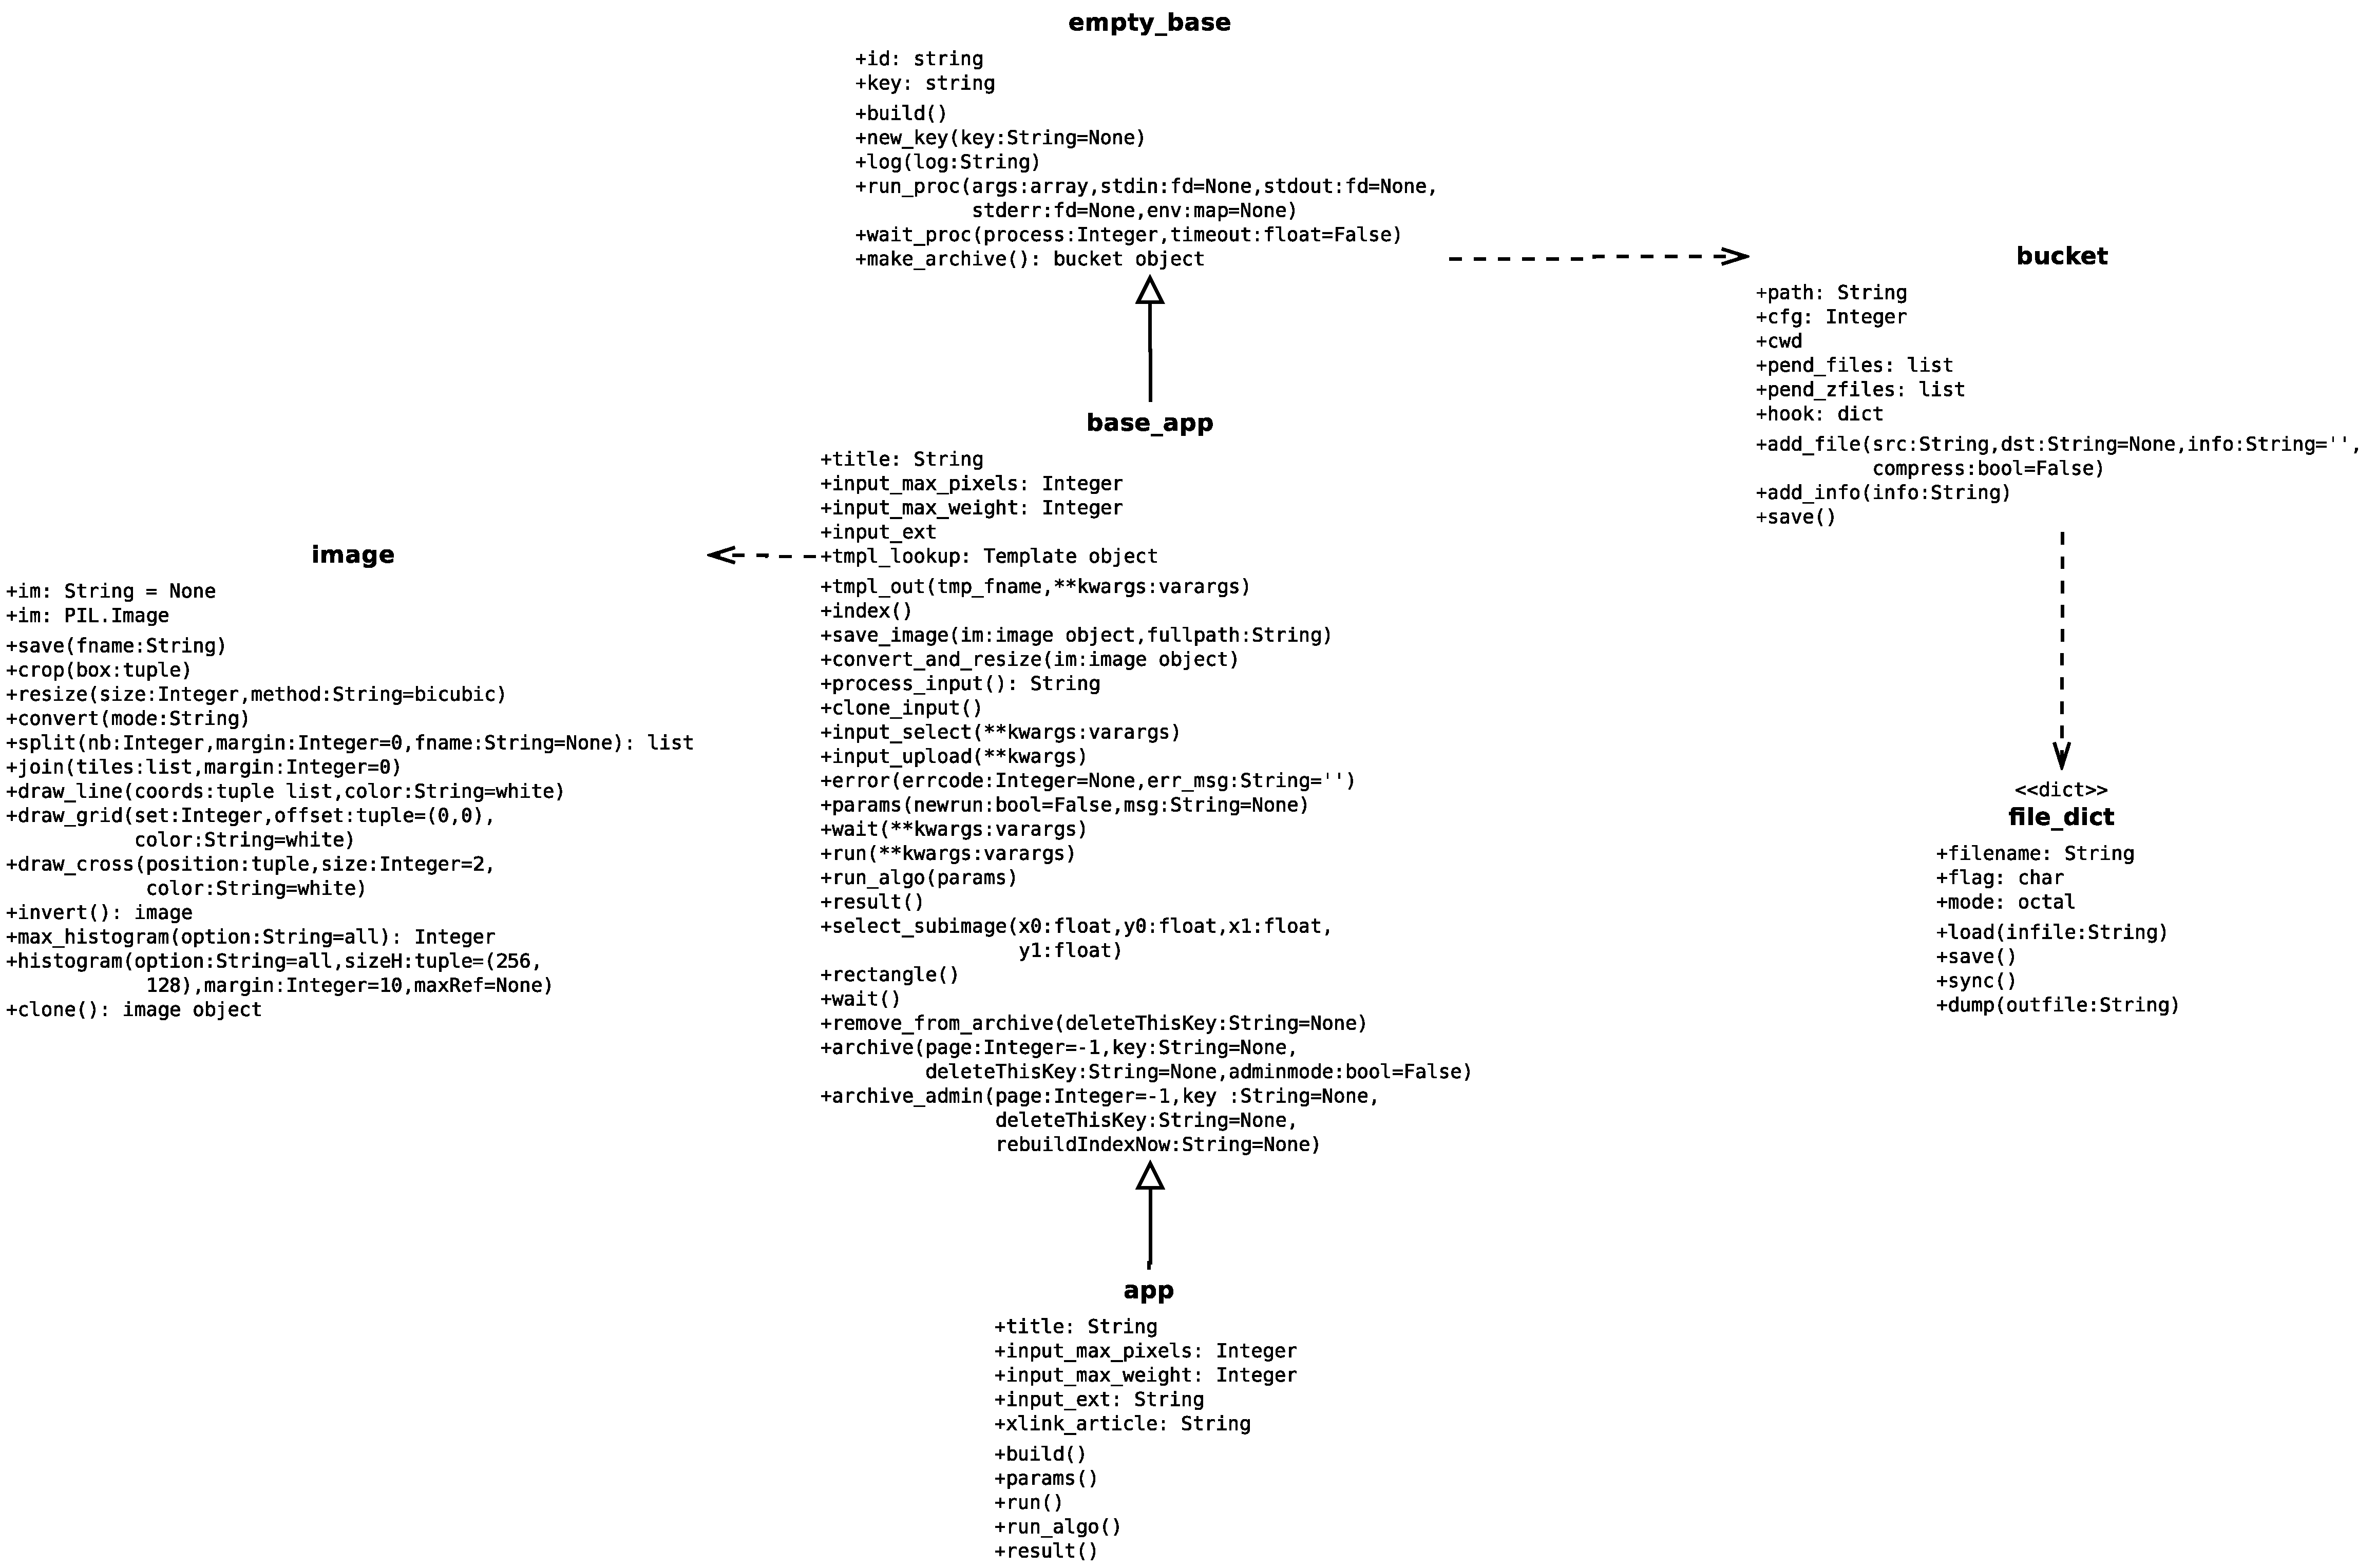
\includegraphics[width=20.0cm, angle=90]{blobs/images/IPOL_diagram_class.pdf}
  \caption{UML diagram class of current system.}
  \label{img:IPOL_diagram_class}
\end{figure}

To conclude this part, images are result of demo and the management of these is important
for the project.

\subsection{Demo}
During introduction, demo system will claim like "God Object". It is excessive term in
order to represent the system with a metaphor. It is just a complex object.
In this section, it will detail functionalities to clarify objective thereof and
look how it is possible to improve it.\\
\setlength{\parindent}{0cm}

Firstly, this object introduce here (\ref{img:IPOL_diagram_class}), has many ways to
interact with user. It implements all features of project. For example, it manages
interaction with client side. To do so, it is a part of webserver developed in
\textbf{CherryPy\footnote{\cite{CherryPy}}}.
Communication between the client and the server is done using an
\textbf{HTTP\footnote{\cite{HTTP}}}. Indeed, when users call a functionality,
this object allows to search the expected result. For example, when users call an algorithm,
it runs the corresponding binary in "bin/" file, manage images archiving the result
and call the HTTP response using the \textbf{Mako Template Library\footnote{\cite{Mako}}}.
Knowing these possibilities, it is very difficult to add new functionalities to this object.
\\
\setlength{\parindent}{0cm}

To conclude this part, the demo is a powerful object but to go further, it needs to create
separate module which communicate with the core system.

\subsection{Solution}
\setlength{\parindent}{1cm}
\hspace{1cm}

Since the problematic have been detailled, it will be necessary to solve it. In this part,
it will present to you \textbf{MVC pattern}, \textbf{Factory pattern}, \textbf{Database}.

\subsubsection{MVC pattern}
\setlength{\parindent}{1cm}
\hspace{1cm}

MVC, alias Model-View-Controller, is architectural pattern used in interface implementation.
It consists of create three separates parts. The model manage database and it is observable
object. The aim of view is to update data from model and to notify event, which by user,
to controler. The controler receive notification from view and update the model.
\setlength{\parindent}{0cm}
In our case, the model will be protocol used to interact with database of images.
The view is client side which look by users using them browser.
It will be updates in the control of the web page on client side.
The controler will be the code used to manage new module implementing functionalities.



\begin{figure}[H]
  \centering
  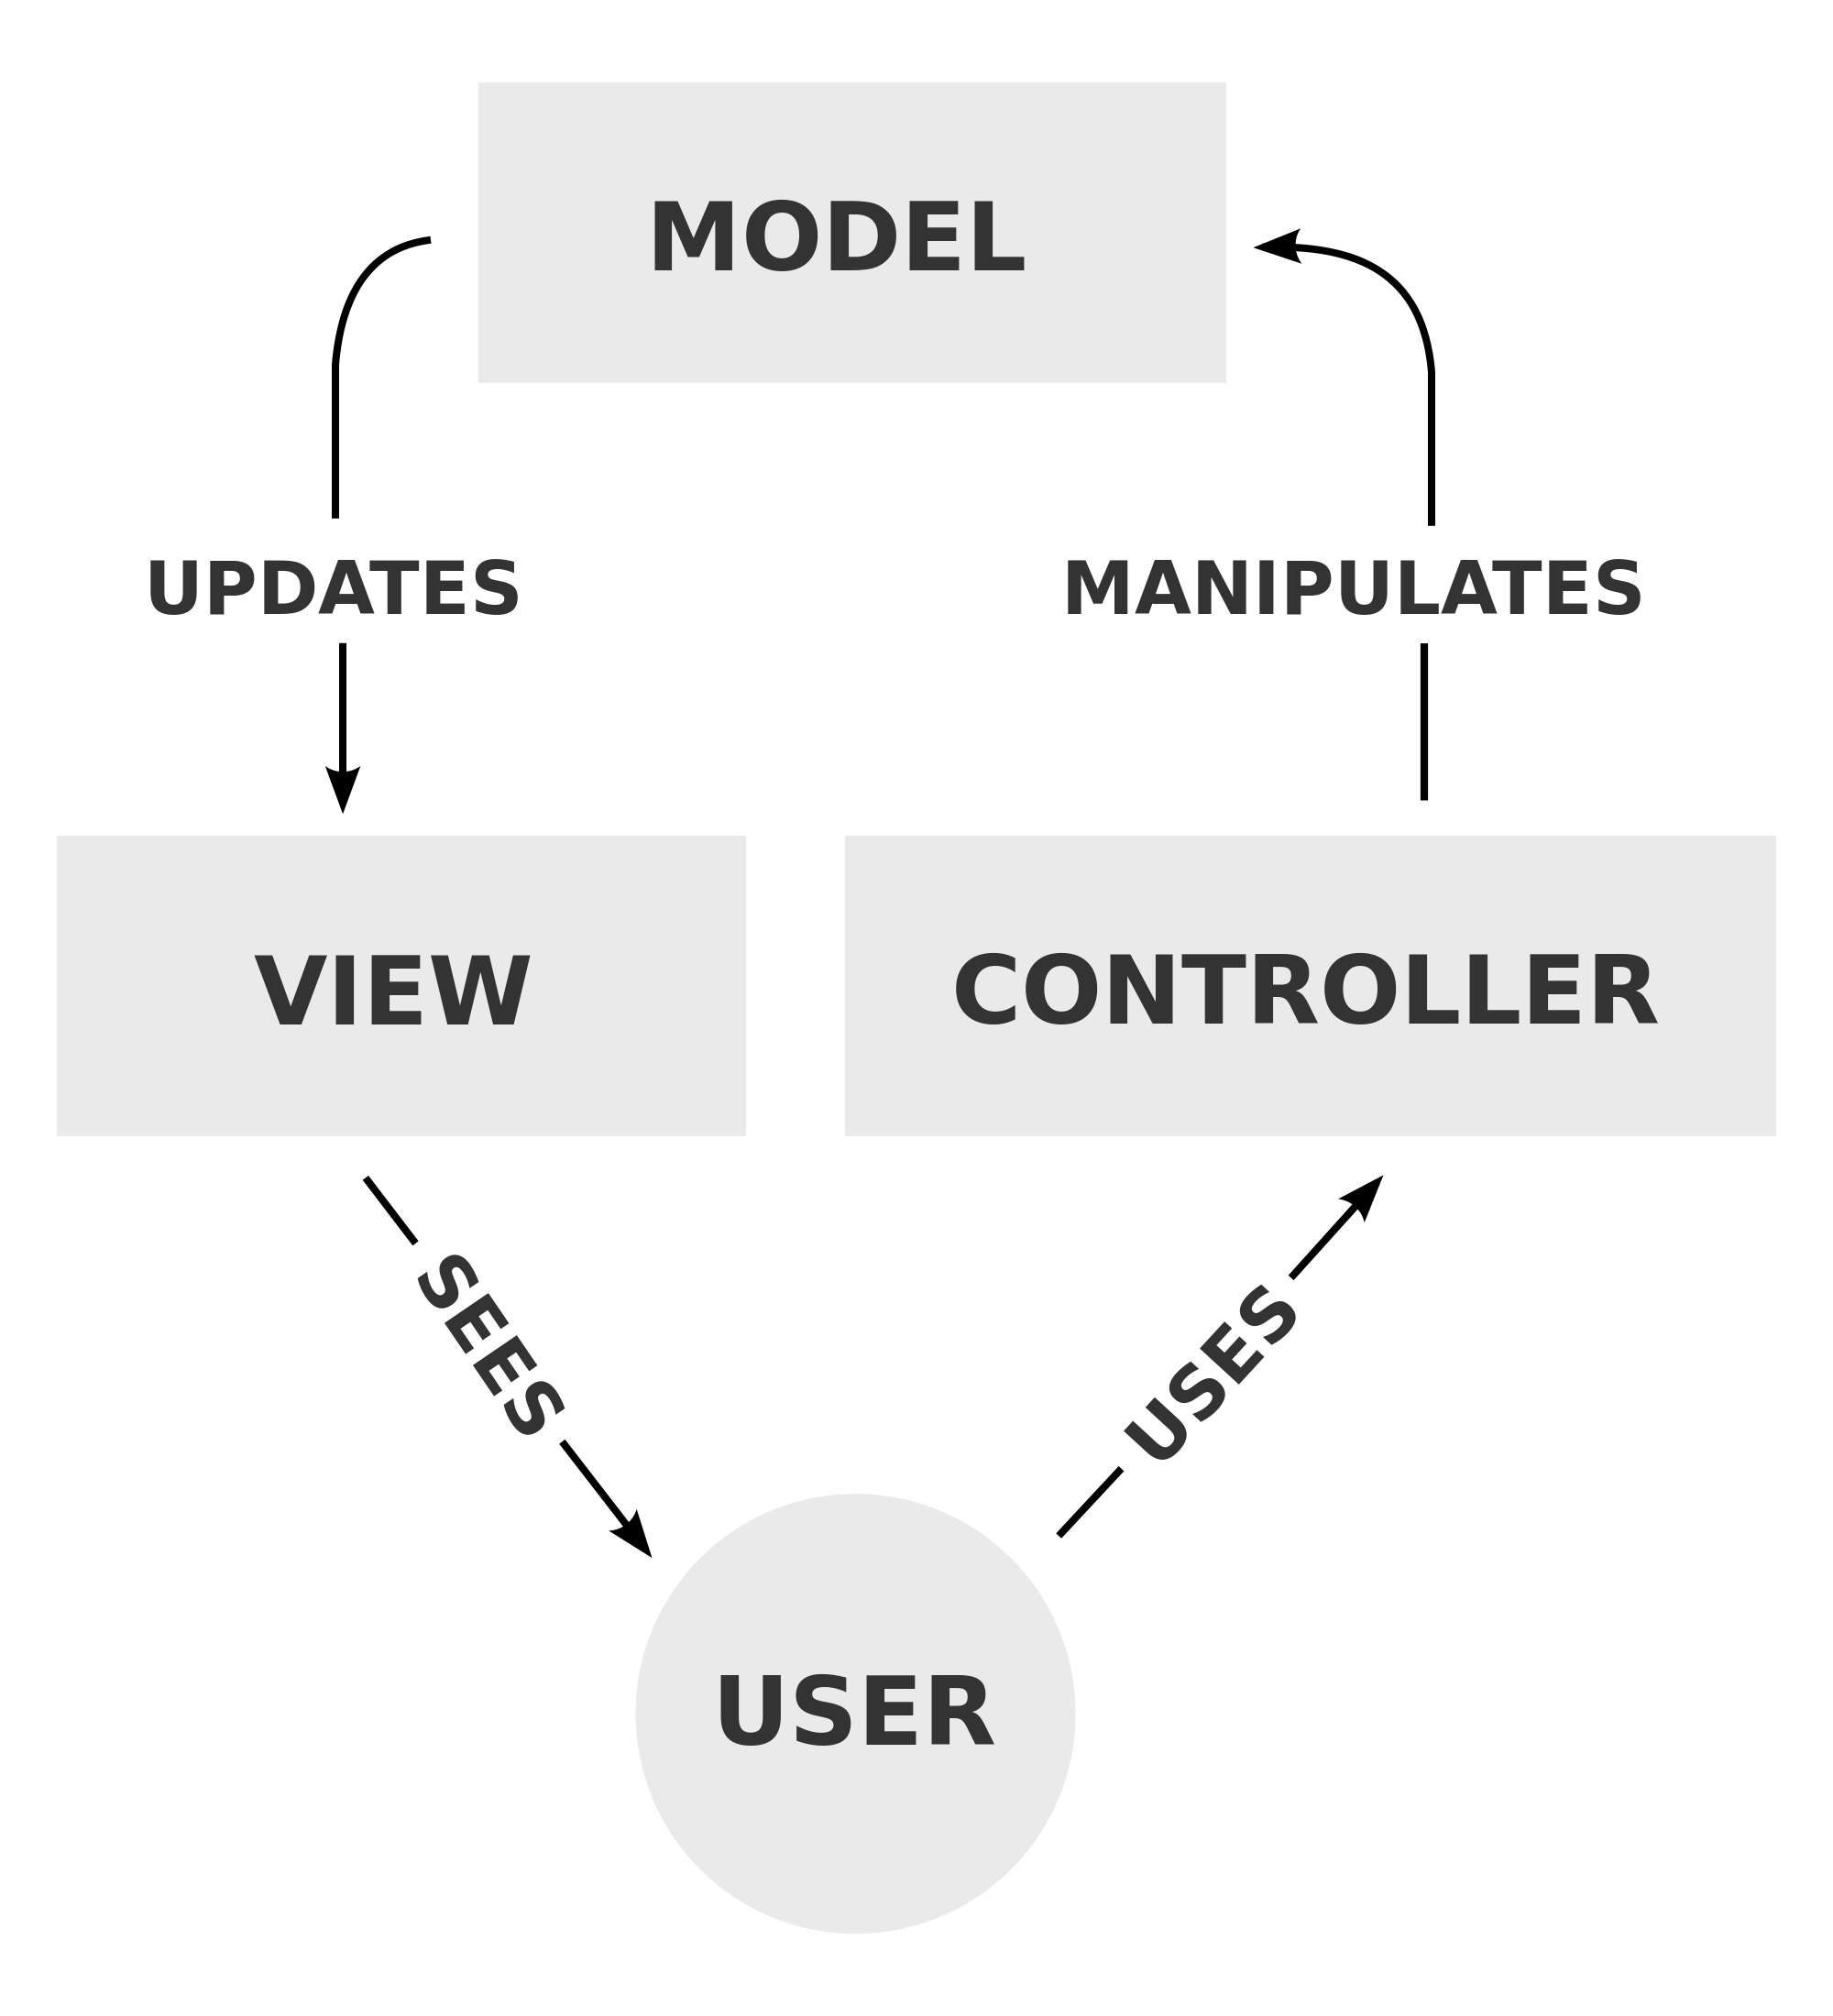
\includegraphics[width=3.5in]{blobs/images/MVC-Process}
  \caption{The MVC pattern}
  \label{img:MVC-Process}
\end{figure}

\subsubsection{Factory pattern}
\setlength{\parindent}{1cm}
\hspace{1cm}
\ToDo{[Miguel] The factory pattern is not used in the new system, since finally
backwards compatibility needs not to be ensure. 
This section should be removed.}

Factory is a \textbf{design pattern\footnote{\cite{GoF}}} allowing to create other objects.
In order to explain the Factory pattern, it must know what is an inheritance.
In inheritance based on object-oriented
programming, it is possible to create an interface (or abstract class) which two different
classes inherit. The most famous example should be the interface Animal which is defined that
Animal could have and it must have to be animal. Dog and Cat are two different classes
inheriting each one from Animal class.
Factory, in this case, could be Farm class. In function to the type of animal which you want
to create (ex: 1 for Cat and 2 for Dog), the Farm will instantiated one of two ways like
Animal class. To do that, it can use implicit or specific cast, it depends of language of
programming.
\bigbreak
\setlength{\parindent}{0cm}
In our case, it will have two versions of demos. The first one like it is nowadays, and the
second one which will be interact with new module. The aim factory is to create just one
object instantiating one of two ways. Consequently, it will be easier to make it work both
version on the same system.

\begin{figure}[H]
  \centering
  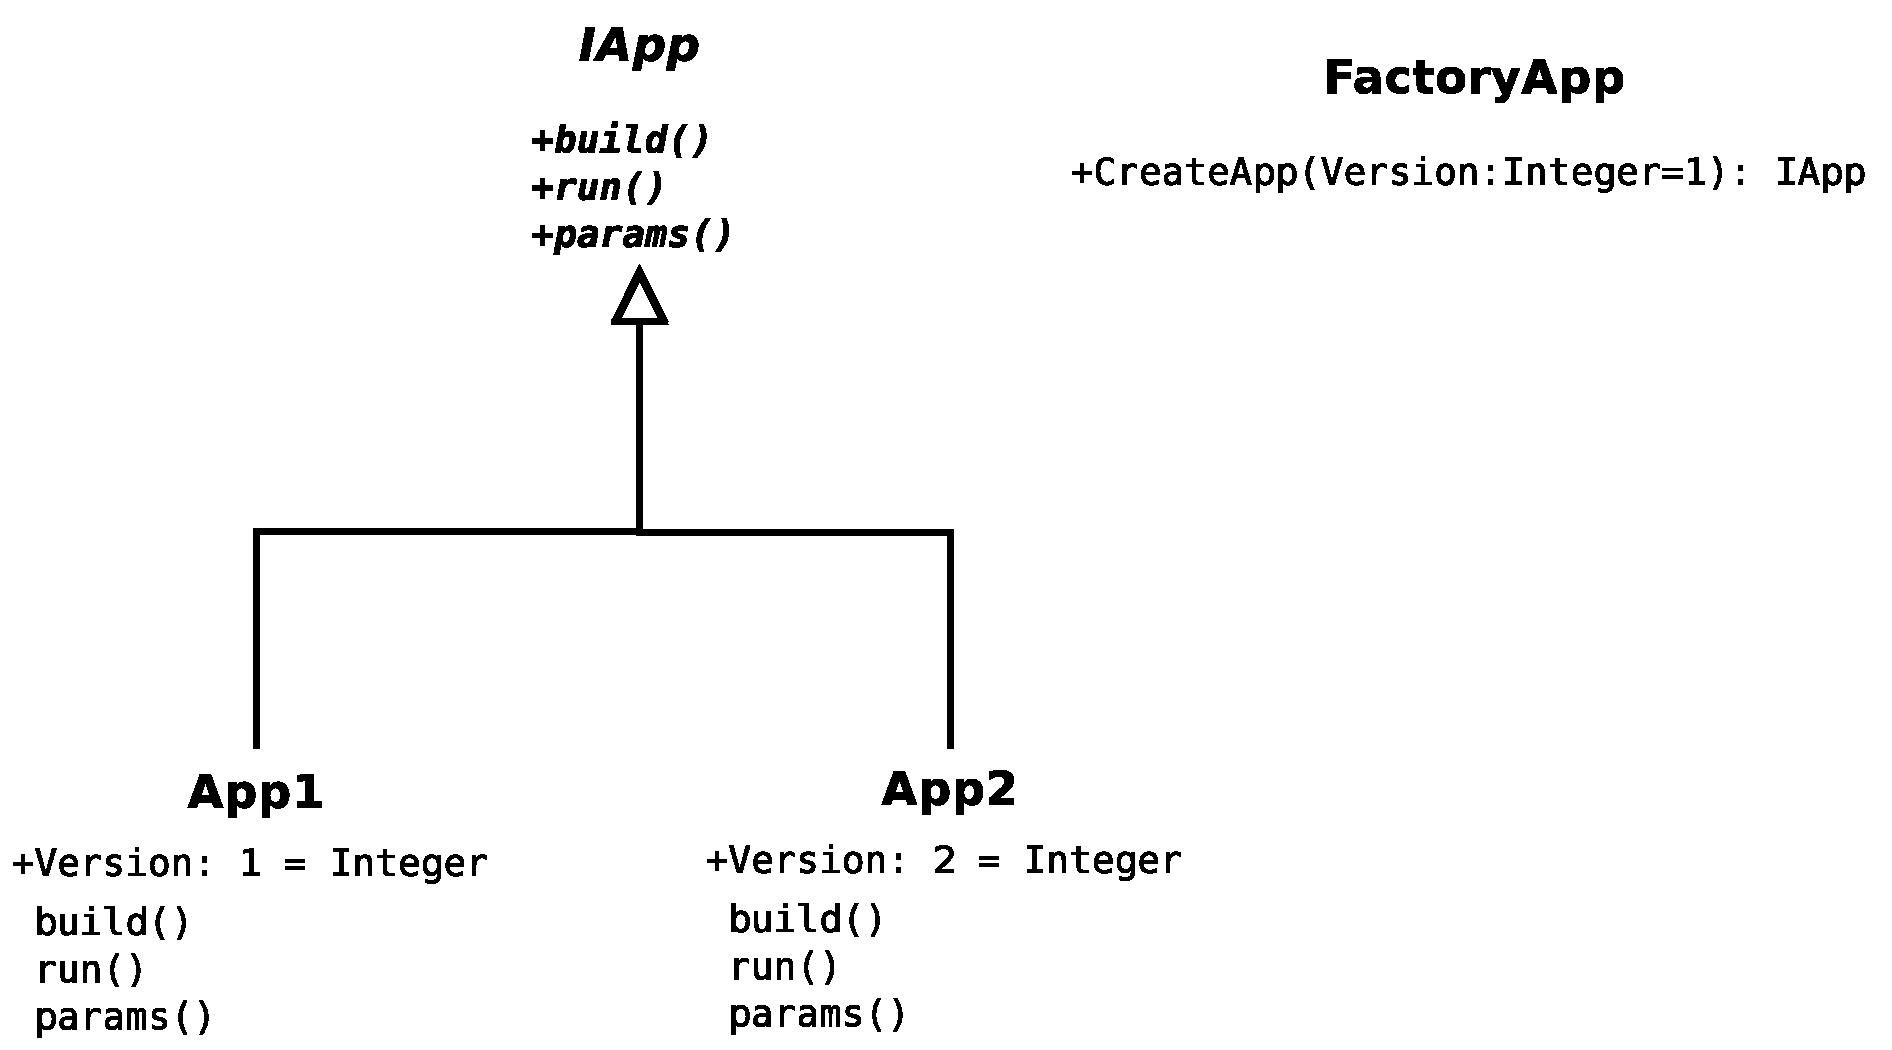
\includegraphics[width=5in]{blobs/images/Example_Factory_Pattern}
  \caption{An example of Factory pattern}
  \label{img:Example_Factory_Pattern}
\end{figure}

\subsubsection{Database}

To solve the problem of images management, it will have a database. It will use a
back-end and will be created with \textbf{SQLite\footnote{\cite{SQLite}}}.
It will have different tables
containing all informations about images. In this way, it will be more easier to
add functionalities and access to images from anything demo. According MVC pattern,
this database will be very useful.\\

\begin{figure}[H]
  \centering
  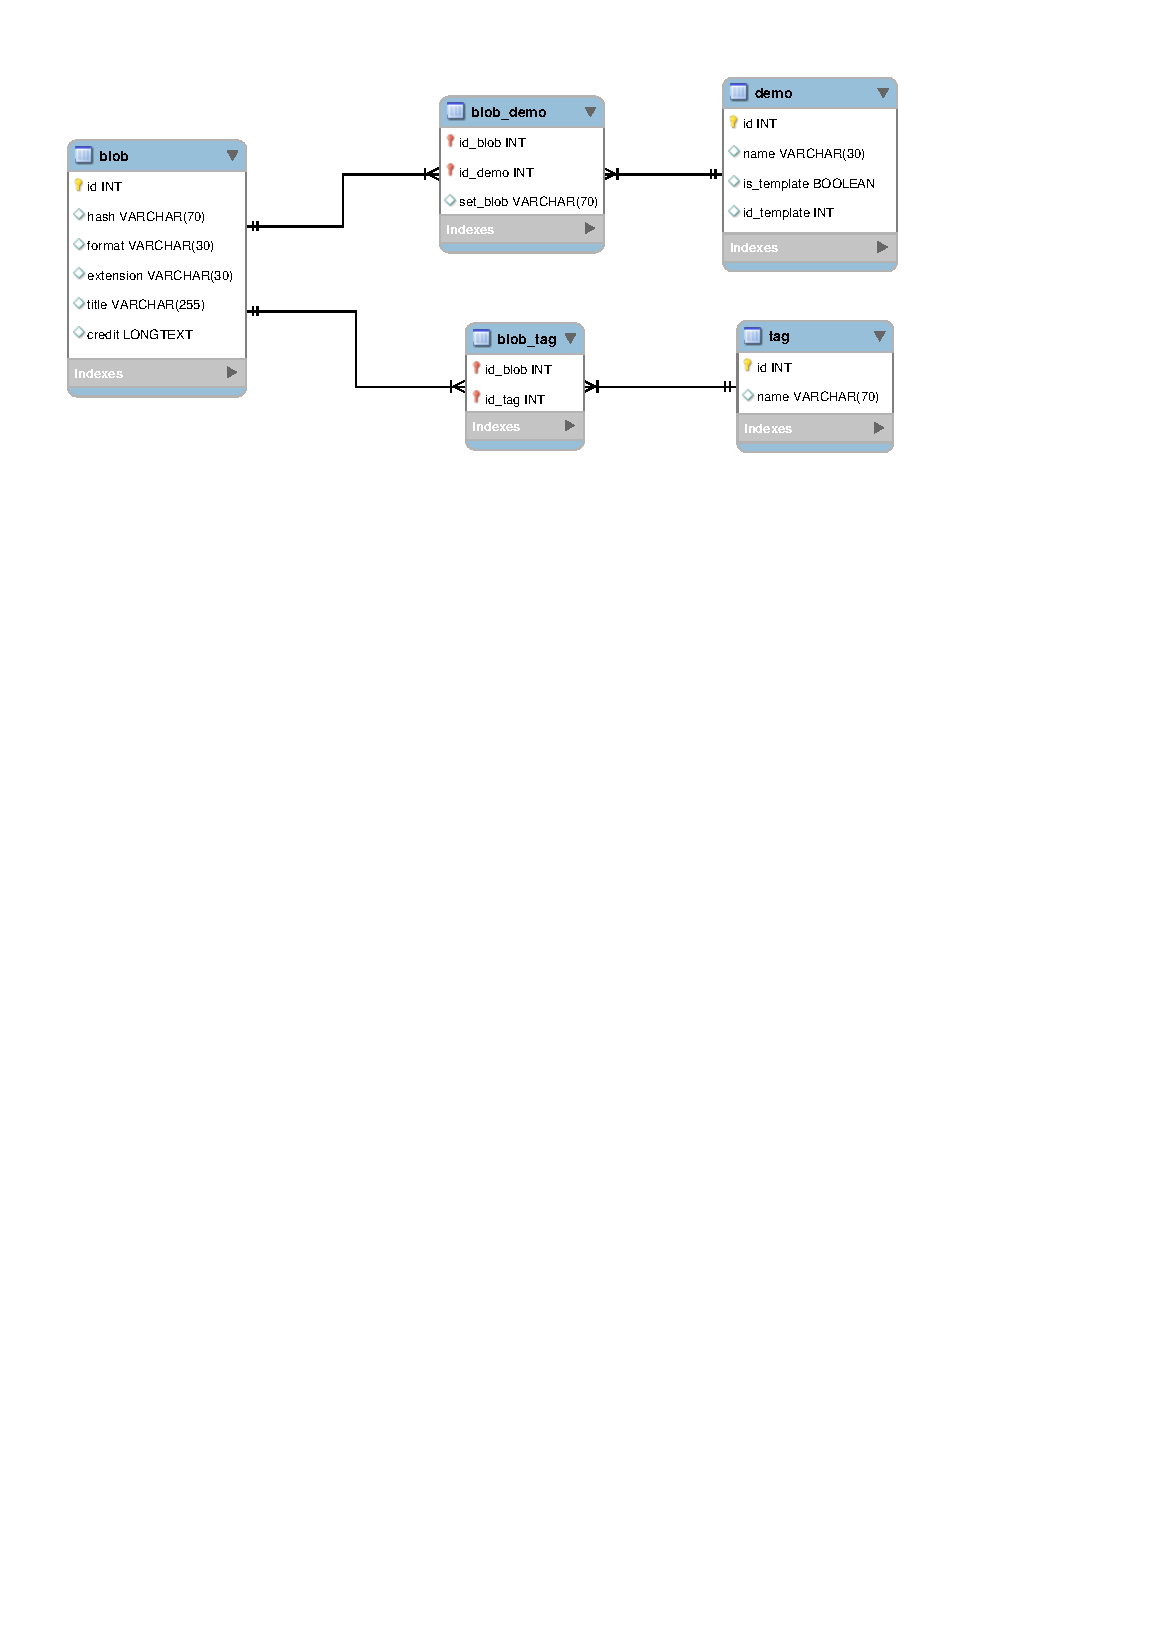
\includegraphics[width=5in]{blobs/images/images_bdd}
  \caption{Database schema for the Blobs module. \ToDo{The image contains a large black at the end and fills out all the page! Fix this.}}
  %\footnotesize
  %\caption*{Realized with MySQL Workbench}
  \label{img:images_bdd}
\end{figure}

\subsection{Remarks}
\subsubsection{Concurrent accesses}
\setlength{\parindent}{1cm}
\hspace{1cm}
The library used to insert, select or update database is
\textbf{SQLite\footnote{\cite{SQLite}}}. This thereof manages, internally,
the concurrent access to database. Indeed, when two people want to
access to the database : the first one will do his request while
the other will be locked by mutex. This principle is also used by transactions
(BEGIN or END/COMMIT).
Therefore, at the beginning of development, it was thought only need a
connection to the database.\\
The problem of the concurrent accesses has been raised during errors occured.
Indeed, when errors occured, the program throws exception and call "roll back"
database's function. Imagine that some people try access to the same data and to
modify it, but some successed it and some failed. The problem of using a only
connection is how to know what changes have been taken into account knowing
that for certain, the database rolled back.\\
Therefore for each request requiring the database,
a new instance (new connection) is used. Thus, the problems
of "roll back" are avoided. Nevertheless, it would be preferable to use a decorator
to avoid the redundance of the code.

\subsubsection{Consistency check}

The consistency check in database management system (DBMS) is the fact
to verify the consistency between the information present on hard disk and
those present on database.\\
There are two ways to do this: running database consistency check manually and
automatically. The program uses consistency check manually in order to
having the control on the error occuring.\\
That is why, when the program uses the action database (SELECT, DELETE, UPDATE),
each information is checked. If errors occurs, an database's exception is caught
and custom exception is throwed to called function.
The consistency check manually is also used because the design databse
has some constraints like: "DELETE CASCADE" and "UPDATE RESTRICT".

\subsubsection{Use case: Web service}
\ToDo{Some of the information here is inconsistent with the actual API implemented in the module. Fix it.}
\ToDo{Think of a better way to describe the webservice API, rather than a table.}

\begin{flushleft}
\begin{longtable}
                   {|C{\dimexpr 0.40\linewidth-2\tabcolsep}
                     ||
                    L{\dimexpr 0.6\linewidth-2\tabcolsep}|}
% {|C{\dimexpr 0.30\linewidth-2\tabcolsep}||
%                     C{\dimexpr 0.20\linewidth-2\tabcolsep}|
%                     C{\dimexpr 0.18\linewidth-2\tabcolsep}|
%                     C{\dimexpr 0.32\linewidth-2\tabcolsep}|}
%   \hline
%   {\bf Function Name} & {\bf Description} & {\bf Param.} & {\bf Return} \tabularnewline
  \hline
  {add\_blob\_ws}
                  & add blob to database \\
                  & {demo\_id path tag ext the\_set title credit} \\
                  & {\{  return:OK or KO, the\_hash: ...  \}} \\
  \hline
  {add\_demo\_ws}
                  & add demo to database \\
                  & {name is\_template template }\\
                  & { \{ return:OK or KO \} }\\
  \hline
  {add\_tag\-\_to\_blob\_ws}
                  & add tag to database \\
                  & { blob\_id tag }\\
                  & { \{ return:OK or KO \} }\\
  \hline
  {delete\_blob\_ws}
                  & delete blob from id demo and id blob \\
                  & {demo\_id blob\_id} \\
                  & { \{ return:OK or KO, delete: (hash, extension) \}} \\
  \hline
  {demos\_ws}
                  & list demos present  in database \\
%                   & { }\\
                  & {\{ return:OK or KO,
                        list\_demos: \{id:name, id\_template, template \} \}} \\
  \hline
  {get\_blob\_ws}
                  & return blob information from id \\
                  & {blob\_id }\\
                  &  {\{ return:OK or KO,
                        \{id, hash,  extension, credit \} \} }\\
  \hline
  {get\_blobs\-\_from\-\_template\_ws}
                  & list blobs from name template \\
                  & {template} \\
                  & { \{ return:OK or KO,
                        blobs: \{id, hash,  extension, format \} \} }\\
  \hline
  {get\_blobs\-\_of\-\_demo\-\_by\_name\_ws}
                  & list blobs from demo name \\
                  & {demo\_name }\\
                  & { \{ return:OK or KO,
                        blobs: \{id, hash,  extension, format \},
                        use\_template: \{id: name, is\_template, id\_template\}\} }\\
  \hline
  {get\_blobs\-\_of\-\_demo\-\_ws}
                  & list blobs from demo id \\
                  & {demo }\\
                  & { \{ return:OK or KO,
                        blobs: \{id, hash,  extension, format \},
                        use\_template: \{id: name, is\_template, id\_template\}\}}\\
  \hline
  {get\_tags\_ws}
                  & return list tags from blob id \\
                  & {blob\_id} \\
                  & { \{ \{id: name\} \} }\\
  \hline
  {get\_tem\-plate\-\_demo\-\_ws} 
                  & return list demos templated \\
                  &  {}\\
                  &  {\{ return:OK or KO, list\_template: \{id: name\} \}} \\
  \hline
  {op\_remove\-\_demo\_ws}
                  & remove demo from id demo  \\
                  & {demo\_id }\\
                  & { \{ return:OK or KO \} }\\
  \hline
  {remove\_tag\-\_from\-\_blob\-\_ws}
                  & remove tag for a blob from id tag and id blob  \\
                  & { id tag\_id blob\_id }\\
                  & { \{ return:OK or KO \} }\\
  \hline
  {set\-\_template\-\_ws}
                  & change the current template used by a demo \\
                  & { demo\_id id name }\\
                  & { \{ return:OK or KO \} }\\
  \hline
\end{longtable}
\end{flushleft}




% The Archive module
\section{The Archive module}
\label{sec:archive}


\subsection{Introduction}
\label{sec:archive_introduction}

%\paragraph{Introduction} \hspace{0pt} \\
The archive module is a standalone application destined to communicate with other modules using webservices. It is designed to implement a stable, simple, and scalable system for archiving all experiments done with IPOL.

\paragraph{Technologies used} \hspace{0pt} \\
The archive module, written in Python, is using fastAPI for webservices, Python Image Library for thumbnails creations, and the python-magic library available on pip (not to be mistaken with python-magic5 which is the one available on the Ubuntu repositories). The module communicates using JSON, both in input and output. The database engine used is SQLite.

\subsection{Architecture}

\paragraph{Module composition} \hspace{0pt} \\
The module is composed of very few files, the code itself in ``archive.py'', a ``router.py'', and a database.

\paragraph{Module architecture} \hspace{0pt} \\
The module is composed of a class, 'Archive', encapsulating the data needed to function. The services offered by the module are all methods of this class. FastAPI will expose all archive http endpoints to make them available and take incoming requests. \\
Upon starting the core module, it will mount archive's router where all endpoints are defined. If they don't exist, both the database and the directories needed for the storage of blobs, logs, the database and thumbnails will be created in their corresponding locations specified in the ``config.py'' file, provided that the user launching the module has the necessary rights. Otherwise, the module will not start. These directories are indicated in the ``config.py'' file, if they are missing from it, the module will not start. \\
The services all connect to each database in a thread-safe way, instanciating its own connection when called, commiting when done if there are modifications, or rollbacking individual queries, if there is an error, and closing the connection. \\
There is a logger initialised with the Archive object, writing errors in ``error.log'' in the logs directory given in the configuration file.

\subsection{Database design}

The database contains 3 tables : experiments, blobs, and correspondence.\\
Each experiments, and each blobs are defined individually, and linked to each-others in the correspondence table, assuring a many-to-many connection. It is worth noting that the database does not save duplicates of the same blob. \\

\ToDo{[Miguel] The right name for the ``correspondence" table is \emph{Junction table}. You can keep the name ``correspondence", but explain in the text that it is a junction table.}

\begin{tabular}{|l|c|r|}
  \hline
  experiments & blobs & correspondence \\
  \hline
  id & id & id \\
  id\_demo & hash & id\_experiment \\
  params & type & id\_blob \\
  timestamp & format & name \\
  \hline
\end{tabular} \\

\paragraph{Experiments table} \hspace{0pt} \\
The experiments table is defined as such : the id field, that stores the unique id of the experiment ; the id\_demo field, that stores the id of the IPOL demo used for the experiment ; the params field, which is a JSON string whose format varies from demo to demo ; and finally the timestamp field.

\paragraph{Blobs table} \hspace{0pt} \\
The blobs table is defined as such : the id field, that stores the unique id of the blob ; the hash field, that stores the hash of the blob computed with sha1, the type field, that stores the extension of the blob (e.g. ``jpeg'' or ``png''), and the format field, that stores the media format of the blob : it is a string, either ``audio'', ``video'' or ``image''. \\
The physical location of a blob is ``blob\_dir as defined in the configuration file'' + ``hash of the blob'' + ``.'' + ``type of the blob''.

\paragraph{Correspondence table} \hspace{0pt} \\
\ToDo{[Miguel] You can keep the name ``correspondence", but explain in the text that it is a junction table.}
The correspondence table is defined as such : the id field ; the id of the experiment and the id of the blob that is linked to said experiment, and the name field, which indicates the role of the blob in the experiment (example : ``input'' or ``denoised''). A foreign key constraint allowing cascade delete is put on the field id\_experiment, referencing the id of an entry in the experiment table, for automatic data deletion.

\ToDo{[Miguel] Why don't we have a FK reference in \emph{correspondence} to link correspondence.id\_blob with blobs.id? It seems that it could be possible to add a row in \emph{correspondence} which refers to a non-existing blob.}

\subsection{Services}

\paragraph{Adding an experiment to the archive} \hspace{0pt} \\
Example :
\begin{verbatim}
http://<localhost>:<port>/add_experiment?demo_id=42&blobs=
<json_blobs>&parameters=<json_parameters>
\end{verbatim}
The method ``add\_experiment'' takes in the entry of the id of the demo used ; a JSON string of the format : 
\begin{verbatim}
{
    url_blob : name,
    ...
}
\end{verbatim}

containing a description of each blob used by and produced by the experiment, with their temporary URLs and names ; and a JSON string describing the parameters of the demo used for the experiment. It will add an experiment to the database by creating a new entry in the experiment table. If the blobs used by and produced by the experiment aren't already in the database, it will copy them in the directory given in the configuration file, and create a thumbnail for the images. It will return a json string containing the status of the operation, OK if it succeeded, KO if there was an error and the operation wasn't performed, as such :

\begin{verbatim}
{
    status : OK/KO
}
\end{verbatim}

If status is KO, a log describing the error will be written.

The following lines area an example og using the archive. 
\begin{verbatim}
http://<localhost>:<port>/add_experiment?demo_id=1000018&blobs=
{"/home/ipol/ipolDevel/ipol_demo/app_new/
1000018/tmp/683D6476AACA4EB929F5D44600AF5F1C/input_0.sel.png": 
"selected subimage", "/home/ipol/ipolDevel/ipol_demo/
app_new/1000018/tmp/683D6476AACA4EB929F5D44600AF5F1C/input_1.png":
"noisy image", "/home/ipol/ipolDevel/ipol_demo/app_new/
1000018/tmp/683D6476AACA4EB929F5D44600AF5F1C/input_0.orig.png": 
"uploaded image", "/home/ipol/ipolDevel/ipol_demo/app_new/
1000018/tmp/683D6476AACA4EB929F5D44600AF5F1C/output_2.png": 
"difference image","/home/ipol/ipolDevel/ipol_demo/app_new/
1000018/tmp/683D6476AACA4EB929F5D44600AF5F1C/output_1.png":
"denoised image"}&parameters={"run time": 0.620905876159668, "sigma": 10}
\end{verbatim}

\paragraph{Deleting an experiment from the archive} \hspace{0pt} \\
When removing an experiment from the database via the method ``delete\_experiment'', every blob linked to this experiment and only to this experiment is removed. After that, all the entries in the correspondence table referencing this experiment are removed automatically due to a foreign key constraint. It return a json response containing the status of the operation of the same format as the return of the method ``add\_experiment''. The method shouldn't be called anywhere else than through the user interface described later.

\paragraph{Deleting a blob from the archive} \hspace{0pt} \\
Due to a many-to-many link between blobs and experiments in the database, a blob has a lot of dependencies : it has of course the experiments using this blobs, but also the blobs linked to these experiments. For deletion of a blob from the archive, the precedent service is called on each experiment the blob is part of, assuring that no orphan data stay in the database (e.g. experiments linked to removed blobs or blobs linked to removed experiments). The method implementing this service is ``delete\_blob\_w\_deps''. It return a json response containing the status of the operation in the same format as the return of the method ``add\_experiment''. The method shouldn't be called anywhere else than through the user interface described later.

\paragraph{Getting data \ToDo{[Miguel] use a more specific word than ``data"} from an archive page} \hspace{0pt} \\
Example :
\begin{verbatim}
http://<localhost>:<port>/page?demo_id=42&page=3
\end{verbatim}
The method ``page'' returns a JSON response with, for a given page of a given demo, all the data of the experiments that should be displayed on this page. Twelve experiments are displayed by page. For rendering the archive page in the browser, the JSON response should be parsed and interpreted in a dedicated template furnished by the front-end of another module. The JSON response is formatted this way : 
\begin{verbatim}
{
    status :  OK/KO,
    experiments : [
        {
            date : timestamp_example, 
            files : [
                {
                    url : url_example,
                    id : id_example,
                    name : name_example,
                    url_thumb : url_thumbnail_example
                }
            ... ],
            id : id_example,
            parameters = {parameters_example...}
    ... ],
    id_demo : id_demo_example,
    nb_pages : nb_pages_example
}
\end{verbatim} 

\paragraph{Shutdown} \hspace{0pt} \\
Example :
\begin{verbatim}
http://<localhost>:<port>/shutdown
\end{verbatim}
The method ``Shutdown'' shuts down the archive application when called. It returns a json response containing the status of the operation.

\paragraph{Other services} \hspace{0pt} \\
Other services features the method ``ping'', simply for checking if the module is up, and the method ``stats'', formatted this way :
\begin{verbatim}
{
    status : OK/KO,
    nb_experiments : x,
    nb_blobs : y
}
\end{verbatim}
Example :
\begin{verbatim}
http://<localhost>:<port>/ping
\end{verbatim}
Example :
\begin{verbatim}
http://<localhost>:<port>/stats
\end{verbatim}

\paragraph{Demo List, a list of all available demos in archive module} \hspace{0pt} \\
Example :
\begin{verbatim}
http://<localhost>:<port>/demo_list
\end{verbatim}
Returns a list of demo ids that have experiments stored in archive module
Returns a  JSON as:
\begin{verbatim}
{status: "OK",demo_list: [125,230]}
\end{verbatim} 


\paragraph{Delete Demo, deletes a demo from archive module} \hspace{0pt} \\
Example :
\begin{verbatim}
http://<localhost>:<port>/delete_demo_w_deps?demo_id=42
\end{verbatim}
Deletes all experiments for a demo.
\begin{verbatim}
{status: "OK/KO"}
\end{verbatim} 

\subsection{Experiment reconstruction}
The IPOL archive reconstruction mechanism allows users to reload archived experiments with the corresponding parameters and eventually run the experiment again. This allows the users to recover a view of the demo page showing the execution of the archived experiment. Note that this mechanism only reads the inputs, parameters and results from the archive, but does not execute again the experiment. 

The information to reconstruct the experiment is obtained with the service that allows to retrieve any stored experiment. Along with the experiment data itself, the response adds also the execution request sent by the client and its response. With this, the client has complete information to render back the experiment page.

To allow the archive reconstruction of a demo, the editor has to specify the field "enable\_reconstruct": true, in the {\tt archive} DDL section. Since all the data for the reconstruction comes from the archived experiment, it is required that the editor ensures that all the needed files are archived in order to reconstruct correctly the demo page without broken images. It might happen that the editor does not want to show in the page of the archive. The "hidden\_files" field it is available to store files in the archive without showing them in the archive page, then they will be only used when the reconstruct happens.

All the stored files must have different names to avoid filename conflicts. 

% The Demo Description Language and automatic demo generation
% Instructions to modify this document:
% * Remember to ALWAYS execute "git pull" BEFORE any commit you make!
% * Use the \ToDo{...} command to remark tasks which still need to be done. Add your name in the comment.
% * Use the \input{file.tex} command to split the document into several parts
% * Do not change the current LaTeX coding style to yours. The style and format should be homogeneous along sections.

% To convert .dia diagrams into PDF:
% 1) Create the diagram with dia
% 2) Export it as .eps
% 3) use epstopdf to convert to PDF
%
% Editing SVG files and exporting them to PDF with Inkscape is admitted too.
% Remember to keep a copy of the editable file (.dia or .svg files).


\documentclass[a4paper,12pt]{article}

\usepackage[utf8]{inputenc}
\usepackage{amsmath,graphicx}
\usepackage{bm}
\usepackage{amssymb}
\usepackage{algorithm}
\usepackage{algpseudocode}
\usepackage{subfigure}
\usepackage{ifpdf}
\usepackage[hyphens]{url}
\usepackage{color}
\usepackage[hidelinks]{hyperref}
\usepackage{multirow}
\usepackage{datetime}
\usepackage{comment}
\usepackage{float} % To put figures in their exact place with \begin{figure}[H]
\usepackage{longtable}
\usepackage{tabularx}
\usepackage{listings}
\usepackage{xcolor}
\usepackage{color}
\usepackage{parskip} % Avoid automatic indentation of every paragraph

\usepackage[most]{tcolorbox}

\definecolor{mygreen}{rgb}{0,0.6,0}
\definecolor{mygray}{rgb}{0.5,0.5,0.5}
\definecolor{mymauve}{rgb}{0.58,0,0.82}

\lstset{ %
  language=HTML,                 % the language of the code
  backgroundcolor=\color{white},   % choose the background color; you must add \usepackage{color} or \usepackage{xcolor}
  basicstyle=\small,        % the size of the fonts that are used for the code
  breakatwhitespace=false,         % sets if automatic breaks should only happen at whitespace
  breaklines=true,                 % sets automatic line breaking
  captionpos=b,                    % sets the caption-position to bottom
  commentstyle=\color{mygreen},    % comment style
  deletekeywords={...},            % if you want to delete keywords from the given language
  escapeinside={\%*}{*)},          % if you want to add LaTeX within your code
  extendedchars=true,              % lets you use non-ASCII characters; for 8-bits encodings only, does not work with UTF-8
  frame=single,                    % adds a frame around the code
  keepspaces=true,                 % keeps spaces in text, useful for keeping indentation of code (possibly needs columns=flexible)
  keywordstyle=\color{blue},       % keyword style
  language=HTML,                 % the language of the code
  otherkeywords={*,...},           % if you want to add more keywords to the set
  numbers=left,                    % where to put the line-numbers; possible values are (none, left, right)
  numbersep=5pt,                   % how far the line-numbers are from the code
  numberstyle=\tiny\color{mygray}, % the style that is used for the line-numbers
  rulecolor=\color{black},         % if not set, the frame-color may be changed on line-breaks within not-black text (e.g. comments (green here))
  showspaces=false,                % show spaces everywhere adding particular underscores; it overrides 'showstringspaces'
  showstringspaces=false,          % underline spaces within strings only
  showtabs=false,                  % show tabs within strings adding particular underscores
  stepnumber=2,                    % the step between two line-numbers. If it's 1, each line will be numbered
  stringstyle=\color{mymauve},     % string literal style
  tabsize=2,                     % sets default tabsize to 2 spaces
  title=\lstname                   % show the filename of files included with \lstinputlisting; also try caption instead of title
}


\definecolor{lightgray}{rgb}{.9,.9,.9}
\definecolor{darkgray}{rgb}{.4,.4,.4}
\definecolor{purple}{rgb}{0.65, 0.12, 0.82}
\lstdefinelanguage{JavaScript}{
  keywords={break, case, catch, continue, debugger, default, delete, do, else, false, finally, for, function, if, in, instanceof, new, null, return, switch, this, throw, true, try, typeof, var, void, while, with},
  morecomment=[l]{//},
  morecomment=[s]{/*}{*/},
  morestring=[b]',
  morestring=[b]",
  ndkeywords={class, export, boolean, throw, implements, import, this},
  keywordstyle=\color{blue}\bfseries,
  ndkeywordstyle=\color{darkgray}\bfseries,
  identifierstyle=\color{black},
  commentstyle=\color{purple}\ttfamily,
  stringstyle=\color{red}\ttfamily,
  sensitive=true
}

\newcolumntype{L}[1]{>{\raggedright\arraybackslash}p{#1}}
\newcolumntype{C}[1]{>{\centering\arraybackslash}p{#1}}
\newcolumntype{R}[1]{>{\raggedleft\arraybackslash}p{#1}}


% Definitions and commands
\def \np{\vskip 0.25 cm}
\def \ap{\vskip 0.15 cm}

% JSON listing (see 
%  http://tex.stackexchange.com/questions/83085/how-to-improve-listings-display 
% -of- json-files)
\colorlet{punct}{red!60!black}
\definecolor{background}{HTML}{EEEEEE}
\definecolor{delim}{RGB}{20,105,176}
\colorlet{numb}{magenta!60!black}

\lstdefinelanguage{json}{
    basicstyle=\footnotesize\ttfamily,
    numbers=left,
    numberstyle=\scriptsize,
    stepnumber=1,
    numbersep=8pt,
    showstringspaces=false,
    breaklines=true,
    frame=lines,
    backgroundcolor=\color{background},
    literate=
     *{0}{{{\color{numb}0}}}{1}
      {1}{{{\color{numb}1}}}{1}
      {2}{{{\color{numb}2}}}{1}
      {3}{{{\color{numb}3}}}{1}
      {4}{{{\color{numb}4}}}{1}
      {5}{{{\color{numb}5}}}{1}
      {6}{{{\color{numb}6}}}{1}
      {7}{{{\color{numb}7}}}{1}
      {8}{{{\color{numb}8}}}{1}
      {9}{{{\color{numb}9}}}{1}
      {:}{{{\color{punct}{:}}}}{1}
      {,}{{{\color{punct}{,}}}}{1}
      {\{}{{{\color{delim}{\{}}}}{1}
      {\}}{{{\color{delim}{\}}}}}{1}
      {[}{{{\color{delim}{[}}}}{1}
      {]}{{{\color{delim}{]}}}}{1},
}


\newcommand{\ToDo}[1]{\textcolor{magenta}{\textbf{[ToDo]} \textbf{#1}}}
\newcommand{\miguel}[1]{\textcolor{magenta}{\textbf{[Miguel]} \textbf{#1}}}


\begin{document}


\begin{titlepage}

\begin{center}
\vspace*{-1in}

\vspace*{0.6in}
\begin{Large}
\textbf{The IPOL Demo Description Lines (DDL)} \\
\end{Large}

\vspace*{0.6in}

\small{Compiled on \today\ at \currenttime}

\vspace*{0.6in}
\rule{80mm}{0.1mm}\\
\vspace*{0.1in}
\end{center}

\end{titlepage}

This document contains the technical documentation for the Demo Description Lines (DDL) for the IPOL Demo System 2.0 for the real-time demos generation from their textual description.

\vspace*{0.6in}

%\maketitle
\newpage

\tableofcontents
\newpage

%\listoffigures
%\newpage

% The Demo Description Lines (DDL) reference
\section{Introduction}
The Demo Description Lines (DDL) define an abstract syntax, written in JSON (JavaScript Object Notation) format, that specifies the IPOL demos. Their main objective is to simplify as much as possible the creation of demos by describing them without the need of writing Python or HTML. This allows fast demo editing in the journal. The following sections describe each of the main keys of the DDL:

\begin{itemize}
  \item \textit{general}: general options (required);
  \item \textit{build}: download and compile the source code (required);
  \item \textit{inputs}: description of the inputs  (optional);
  \item \textit{params}: description of the parameters and user control (optional);
  \item \textit{run}: script or binary which needs to be called for the execution, along with its parameters (required);
  \item \textit{archive}: which parameters and files will be stored in the archive (optional);
  \item \textit{results}: which elements will be displayed as results (required).
\end{itemize}

\vspace{1em}

The IPOL control panel provides a JSON editor with a simple validator. Most of the syntax errors are detected in real time and reported by this graphical tool.

%-------------------------------------------------------------------------------
\section{The \emph{general} section}
The general section describes global information about the demo. It is a set of (key, value) pairs, described in the following table. The column \emph{req} refers to a required field. This type of tables will be used in all the sections of this document.

% 
\begin{longtable}{|>{\bf}L{\dimexpr 0.28\linewidth}|L{\dimexpr 
0.57\linewidth}|c|}
\hline
 \centering {key}     & \centering {\bf description} & {\bf req} 
\tabularnewline \hline \hline
 demo\_title         & Title of the demo. & no\\ \hline
 description         & Description to be shown at the beginning of the demo page. It contains HTML or plain text as a single string. & no \\ \hline
 input\_description  & Description of the inputs. It contains HTML as a single string or as an array of string that will be concatenated and separated with spaces. & no \\ \hline
 param\_description  & Description for the parameters. It contains HTML code as a single string or as an array of string that will be concatenated and separated with spaces. & no
\\ \hline
 xlink\_article     & Link to the article webpage & no  \\ \hline
 requirements 	    & It specifies particular requirements needed for the execution of the demo, separated by commas. e.g. Matlab. & no \\ \hline
 custom\_js 	    & It allows to give the URL of a custom Javascript file. This script contains extra JS code that allows to personalize the interaction and look of the front-end. It should only be used in very special cases there there is not any other alternative than overwriting the default behavior or look. & no \\ \hline
 timeout 	    & It specifies maximum time in seconds allows to execute the algorithm. If the execution takes longer than the specified time the system stops the exection. & no \\ \hline
\caption{Fields in the \emph{general} section.}
\end{longtable}

%-------------------------------------------------------------------------------
\section{The \emph{build} section}

The build section is a set of one or more sets, each one providing information to obtain and compile the source codes needed for a given demo. If the demo needs to compile several files from different links, the build sets must be indexed as build1, build2,..., build\textit{n} being \textit{n} the total number of builds (see the example below). It is mandatory to write at least build1. If a demo needs to make use of a python package in order to execute the user will have to specify the requirements.txt file location inside the source binary compressed file. Three steps are needed to build a demo: 

\begin{itemize}
  \item Download the original sources codes (with optional userid and password for private demos);
  \item Build the executables after the download;
  \item Copy the needed files in a run context to execute the  demo.
\end{itemize}

\begin{longtable}{|>{\bf}L{\dimexpr 0.25\linewidth}|L{\dimexpr 0.6\linewidth}|c|}
\hline
\centering {key}     & \centering {\bf description} & {\bf req} \tabularnewline 
\hline \hline
 url        & Link to download the source codes as a compressed file. & yes \\ \hline
 username   & Username for private demos. & no \\ \hline
 password   & Password for private demos. & no \\ \hline
 construct  & Shell command needed to compile the downloaded source code. & no  \\ \hline
 move       & List of files needed to execute the demo separated with commas (see example below) & yes  \\ \hline
 virtualenv & Creates a python 3 virtualenv to install any needed python package inside the bin folder. & no  \\ \hline
\caption{Build fields}
\end{longtable}

\paragraph{Example:}
In this case, the demo needs to compile from two different compressed files. The DDL uses the \textit{move} statement to copy the obtained files after the compilation into a run context.%\\
\begin{lstlisting}[language=json,firstnumber=1]
"build": {
    "build1": {
        "url": "http://www.ipol.im/pub/art/2014/82/sift_anatomy_20141201.zip",
        "construct": "cd sift_anatomy_20141201 && make",
        "move": "sift_anatomy_20141201/bin/sift_cli, sift_anatomy_20141201/bin/match_cli"
    },
    "build2":{
        "url": "http://dev.ipol.im/~monasse/orthoPose_1.0.tar.gz",
        "construct": "matlab -nodisplay -nosplash -nodesktop -r \"cd orthoPose_1.0/; mcc -m mainPoseEstimation.m -a lib/; exit;\"",
        "move": "orthoPose_1.0/mainPoseEstimation, orthoPose_1.0/run_mainPoseEstimation.sh"
        "virtualenv": "sift_anatomy_20141201/requirements.txt"
    }
}
\end{lstlisting}

%-------------------------------------------------------------------------------
\section{The \emph{inputs} section}
The inputs section describes the characteristics of the input data for the algorithm.

\subsection{image}

\begin{longtable}{|>{\bf}L{\dimexpr 0.26\linewidth}|L{\dimexpr 0.59\linewidth}|c|}
\hline
\centering {key}     & \centering {\bf description} & {\bf req} \tabularnewline 
\hline \hline
 type         & type of the input: image & yes \\ \hline
 description  & Short name or description. This is used by the web interface. & no \\ \hline
 max\_pixels  & This value sets the maximum number of pixels allowed for the input. If the size of the image is over this the limit it will be resized. The value can be a number or an arithmetic expression (ex:  ``1000*1000" = 1 Mpx).  & yes \\ \hline
 max\_weight   & Maximum weight (in bytes) of an input file. This prevents uploading too large files. The value can be a number or an arithmetic expression (ex: ``100*1024*1024"= 100 Mb). & no \\ \hline
 dtype        & Final format for the image. Some examples:
\begin{itemize}
  \setlength\itemsep{-0.5em}
  \item \textit{1x8i}: gray, unsigned integer 8 bits;
  \item \textit{3x8i}: color, RGB unsigned integer 8 bits;
  \item \textit{1x16i}: gray, unsigned integer 16 bits;
  \item \textit{3x16i}: color, RGB unsigned integer 16 bits.
\end{itemize} 
 & yes \\ \hline
 ext          & input extension (ie. file format) & yes \\ \hline
forbid\_preprocess & Must be a boolean value. Forbids any pre-processing of the input data.
Submitted image is kept as-is. Used by algorithms like noise estimation or modification detection, where re-sampling will affect results. 
If a processing is needed according to the expected properties, an error message will be displayed to the user. This will also remove the crop feature from the interface.
& no \\ \hline
 control & String to include an interactive control. Possible values are "mask", "dots" and "lines" each for a different kind of mask drawing behaviour. & no \\ \hline
\caption{Fields for an \emph{image} as input.}
\end{longtable}

\subsection{video}

\begin{longtable}{|>{\bf}L{\dimexpr 0.26\linewidth}|L{\dimexpr 0.59\linewidth}|c|}
\hline
\centering {key}     & \centering {\bf description} & {\bf req} \tabularnewline 
\hline \hline
 type         & type of the input: video & yes \\ \hline
 description  & Short name or description. This is used by the web interface. & no \\ \hline
 as\_frames & Boolean value. The input video will be converted to png images for each frame according to the max\_frames field. Frames
 will be stored in a temporal folder inside the execution directory with the name. (ex: ./input\_0/frame\_000.png ) & no \\ \hline
 max\_pixels   & This value sets the maximum number of pixels allowed for the input video per frame. If the size of the input is over, the video frames will be resized. The value can be a number or an arithmetic expression (ex: ``1000*1000" = 1 Mpx).  & yes \\ \hline 
 max\_frames  &  Maximum number of frames after conversion, either as frames or video.  & yes \\ \hline
 max\_weight   & Maximum weight (in bytes) of an input file. This prevents uploading too large files. The value can be a number or an arithmetic expression (ex: ``100*1024*1024"= 100 Mb). & no \\ \hline
forbid\_preprocess & Forbids any pre-processing of the input data by the IPOL system. Submitted video is kept as-is. Used by algorithms like noise-estimation or modification detection, where re-sampling will affect results.If a processing is needed according to the expected properties, an error message will be displayed to the user.
& no \\ \hline
\caption{Fields for a \emph{video} as input.}
\end{longtable}


\subsection{data}

The \emph{data} type is used when the input type is other than an image or a video. Submitted data is kept as it is. The extension of your data file should be defined in the "ext" column. 
\begin{longtable}{|>{\bf}L{\dimexpr 0.26\linewidth}|L{\dimexpr 0.59\linewidth}|c|}
\hline
\centering {key}     & \centering {\bf description} & {\bf req} \tabularnewline 
\hline \hline
 type         & type of the input: data & yes \\ \hline
 description  & Short name or description. This is used by the web interface. & no \\ \hline

 max\_weight   & Maximum weight (in bytes) of an input file. This prevents uploading too large files. The value can be a number or an arithmetic expression (ex: ``100*1024*1024"= 100 Mb). & no \\ \hline

 ext          & input extension (ie. file format, eg: .txt, .tiff) & yes \\ \hline

\caption{Fields for the \emph{data} as input.}
\end{longtable}

\paragraph{Example:}
An example of the \emph{data} input for a demo is shown below. An input file with the .txt format is required in this case.
\begin{lstlisting}[language=json,firstnumber=1]
"inputs": [
    {
    "description": "Text file containing the curve points",
    "max_weight": 524288000,
    "ext": ".txt",
    "required": true,
    "type": "data"
    }
]
\end{lstlisting}

\subsection{map}
The \emph{map} type the interface makes the demo show a map of the Earth where the user can drawn one or more polygons interactively. The selection is passed to the demo's code as a list of GeoJSON features containing geometric coordinates.

\begin{figure}[h]
\centering
\tcbox[sharp corners, boxsep=0.0mm, boxrule=0.5mm, colback=white]{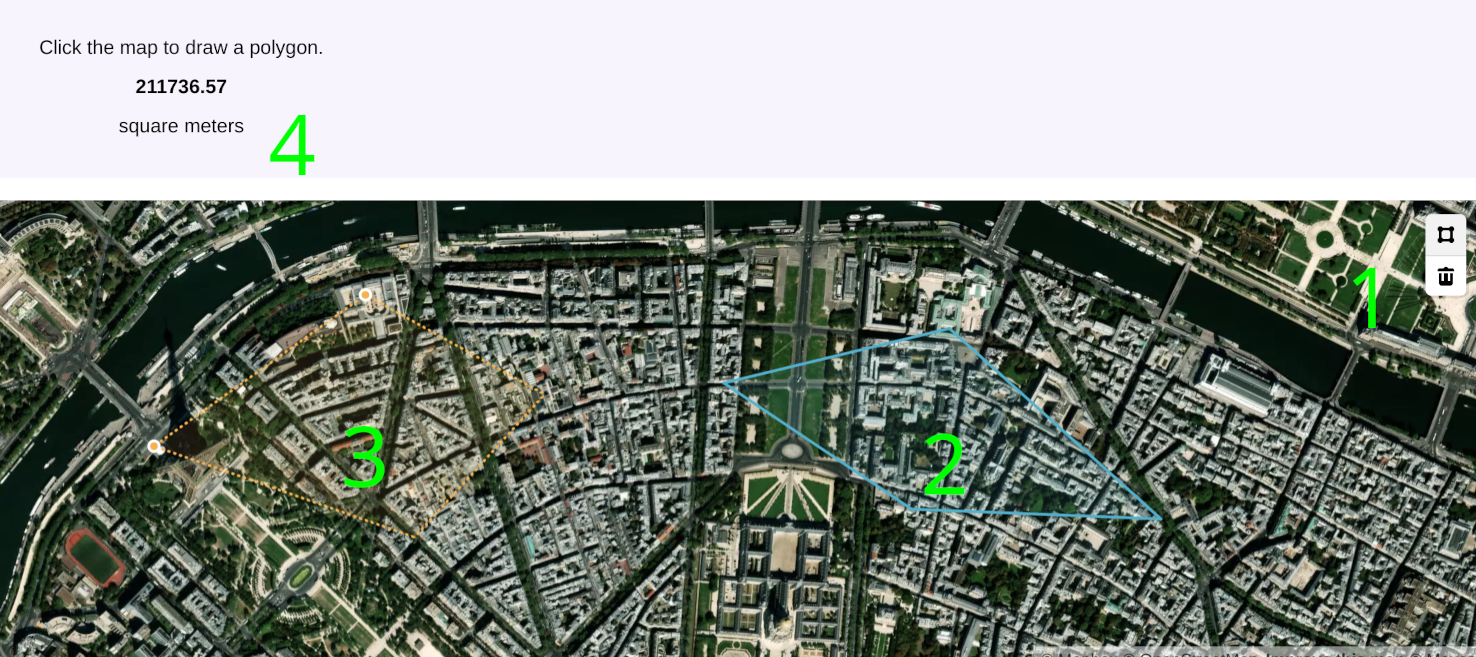
\includegraphics[scale=0.25]{Images/geojson_example.png}}
\caption{The IPOL's map interface. 1) The controls to draw and remove polygons, 2) A polygon already draw, 3) A polygon being drawn, and 4) the information about the current polygon.}
\label{fig:geojson_example}
\end{figure}

Figure~\ref{fig:geojson_example} shows the control and its key elements.
To draw a polygon there is a toolbox (1) which allows to start drawing a polygon and to remove completely the last one. Click on the upper icon to start drawing and click on the map to add as many vertices as needed. You can also start adding vertices by clicking the right button of the mouse. When done, click the right button of the mouse. After that, the polygon will appear as finished (2). You can drawn more than one polygon, if needed. After finishing with the first, you can draw a second one (3). The information about the current polygon is show above (4).

The demo will receive a GeoJSON file containing the coordinates as a list of geometric features. Please check the code of demo 11111000001 to see an example on how to parse the GeoJSON file to extract the geometric coordinates.

The map is an interactive 3D projection. You can move around and change the location using the mouse and dragging with the left button, or using the keyboard cursors. With the right button of the mouse you can rotate the map and change the orientation of the camera. The zoom can be adjusted with the wheel of the mouse or with '+'/'-' in the keyboard.

When a demo uses a map, it can only contain that single input in the DDL.

\begin{longtable}{|>{\bf}L{\dimexpr 0.26\linewidth}|L{\dimexpr 0.59\linewidth}|c|}
\hline
\centering {key}     & \centering {\bf description} & {\bf req} \tabularnewline 
\hline \hline
 type         & type of the input: map & yes \\ \hline
 center         & longitude and latitude (example: [-3.703790, 40.416775] to center the map in Madrid) & no \\ \hline
 ext          & input extension (for example, .json) & yes \\ \hline
\caption{Fields of \emph{map} input type.}
\end{longtable}



%-------------------------------------------------------------------------------
\section{The \emph{params} section}
The \emph{params} section describes the set of parameters needed by a demo, their constraints and the visual appearance of the user control. It is defined as an array of sets, where each set contains (key, value) pairs. In this section, we show examples of the expected appearance of these parameters in the web interface. The look of the controls might differ depending on the operating system and the browser used.

\subsection{range}

The \emph{range} type is used as an horizontal slider constrained by a minimum and a maximum numeric values. It can be moved with the mouse or by using the arrow keys according to the step value fixed in the DDL. The user control is similar to the one at Figure~\ref{fig:sliders}.

\begin{longtable}{|>{\bf}L{\dimexpr 0.15\linewidth}|L{\dimexpr 
0.7\linewidth}|c|}
\hline
 \centering {key}     & \centering {\bf description} & {\bf req} 
\tabularnewline \hline \hline
 type   & range       & yes \\ \hline
 id     & Used to identify the parameter. & yes \\ \hline
 label  & A name and/or description of the parameter. It appears on the left side in the web interface. & no
                      \\ \hline
 comments & A description of the parameter. It appears on the right side in the web interface. & no
                      \\ \hline
 visible    & Javascript expression evaluated as a boolean. & no \\ \hline
 values & Sets min, max, step and default values using a key/value 
scheme \{ "min":val, "max":val, "step":val, "default":val \}. 
Ex: to select a value included in (-1, -0.5, 0, 0.5, 1) write \texttt{"values": \{"min": -5, "max": 5, "step": 0.5, "default": 0\}}  & yes
                      \\ \hline
\caption{Fields for the properties of the \emph{range} type.}
\end{longtable}

\begin{figure}[h]
\centering
\tcbox[sharp corners, boxsep=0.0mm, boxrule=0.5mm, colback=white]{\includegraphics[scale=0.35]{Images/slider_examples.png}}
\caption{Range type example. It shows a slider with values from 0.02 to 0.2.}
\label{fig:sliders}
\end{figure}

\subsection{selection\_collapsed}

The \emph{selection\_collapsed} type returns one string selected by a key (for example, a color code selected by name). The user control is a dropdown select similar to the one in Figure~\ref{fig:selection_collapsed_example}.

\begin{longtable}{|>{\bf}L{\dimexpr 0.25\linewidth}|L{\dimexpr 
0.6\linewidth}|c|}
\hline
 \centering {key}     & \centering {\bf description} & {\bf req} 
\tabularnewline \hline \hline
 type  & selection\_collapsed    & yes \\ \hline
 id     & Used to identify the parameter. & yes \\ \hline
 label  & A name and/or description of the parameter. It appears on the left side in the web interface. & no
                      \\ \hline
 comments & A description of the parameter. It appears on the right side in the web interface. & no
                      \\ \hline
 visible    & Javascript expression evaluated as a boolean.
            & no \\ \hline
 values & set of (key, value) pairs, where the key is the displayed text and the 
value is the string returned, for example \texttt{"values": \{"black": "000000", "white": "FFFFFF"\}} & yes
                      \\ \hline
 default\_value & defines the default value for this parameter, should be one 
the values defined in 'values'. & yes \\ \hline
\caption{Fields for the properties of the \emph{selection\_collapsed} type.}
\end{longtable}

\begin{figure}[h]
\centering
\tcbox[sharp corners, boxsep=0.0mm, boxrule=0.5mm, colback=white]{\includegraphics[scale=0.35]{Images/selection_collapsed_example.png}}
\caption{Selection collapsed example. In this case, the selection offers five options to choose.}
\label{fig:selection_collapsed_example}
\end{figure}

\clearpage
\subsection{selection\_radio}

The \emph{selection\_radio} returns one string selected by a key (for example, a color code selected by name). The user control is a set of radio buttons as in Figure~\ref{fig:selection_radio_example}.

\begin{longtable}{|>{\bf}L{\dimexpr 0.25\linewidth}|L{\dimexpr 
0.6\linewidth}|c|}
\hline
 \centering {key}     & \centering {\bf description} & {\bf req} 
\tabularnewline \hline \hline
 type     & selection\_radio    & yes \\ \hline
 id     & Used to identify the parameter. & yes \\ \hline
 label  & Name and/or description of the parameter. It appears on the left side in the web interface. & no
                      \\ \hline
 comments & Description of the parameter. It appears on the right side in the web interface. & no
                      \\ \hline
 visible    & Javascript expression evaluated as a boolean.
            & no \\ \hline
 values   & set of (key, value) pairs, where the key is the displayed text and the 
value is the string returned, for example \texttt{"values": \{"black": "000000", "white": "FFFFFF"\}} & yes
                      \\ \hline
 default\_value & defines the default value for this parameter, should be one 
the values defined in 'values'. & yes \\ \hline
 vertical & It is boolean value. The button distribution is vertical when the value is activated (true), otherwise, the visualization is horizontal as default. & no \\ \hline
\caption{Fields for the properties of the \emph{selection\_radio} type.}
\end{longtable}

\begin{figure}[h]
\centering
\tcbox[sharp corners, boxsep=0.0mm, boxrule=0.5mm, colback=white]{\includegraphics[scale=0.35]{Images/selection_radio_example.png}}
\caption{Radio buttons example. The label description is Mode and the parameter offers two radio buttons. The vertical option is disabled.}
\label{fig:selection_radio_example}
\end{figure}

\subsection{label}

The \emph{label} type can be used to separate groups of parameters or to include html fields (images, external links, etc.) in the web interface.

\begin{longtable}{|>{\bf}L{\dimexpr 0.27\linewidth}|L{\dimexpr 
0.58\linewidth}|c|}
\hline
 \centering {key}     & \centering {\bf description} & {\bf req} 
\tabularnewline \hline \hline
 type  & label       & yes \\ \hline
 label & HTML text to display, as a single string or as an array of strings. & yes \\ \hline
 visible    & Javascript expression evaluated as a boolean.
            & no \\ \hline
\caption{Fields for the properties of the \emph{label} type.}
\end{longtable}

\begin{figure}[h]
\centering
\tcbox[sharp corners, boxsep=0.0mm, boxrule=0.5mm, colback=white]{\includegraphics[scale=0.30]{Images/label_example.png}}
\caption{Label example. The label explains that the sliders below represent matrix values according to the image depicted in the label.}
\label{fig:label_example}
\end{figure}

\subsection{checkbox}

The \emph{checkbox} type returns a boolean value. The user control is a checkbox similar to the one in Figure~\ref{fig:checkbox_example}.

\begin{longtable}{|>{\bf}L{\dimexpr 0.27\linewidth}|L{\dimexpr 
0.58\linewidth}|c|}
\hline
 \centering {key}     & \centering {\bf description} & {\bf req} 
\tabularnewline \hline \hline
 type  & checkbox  & yes \\ \hline
 id     & Used to identify the parameter. & yes \\ \hline
 label  & A name and/or description of the parameter. It appears on the left side. & no
                      \\ \hline
 comments & A description of the parameter. It appears on the right side in the web interface. & no
                      \\ \hline
 visible    & Javascript expression evaluated as a boolean. & no \\ \hline
 default\_value & boolean: True for checked & \\ \hline
\caption{Fields that manages the properties of the \emph{checkbox} type.}
\end{longtable}

\begin{figure}[h]
\centering
\tcbox[sharp corners, boxsep=0.0mm, boxrule=0.5mm, colback=white]{\includegraphics[scale=0.35]{Images/checkbox_example.png}}
\caption{Checkbox example. This can be used in the demos that need to activate or not an option.}
\label{fig:checkbox_example}
\end{figure}

\subsection{numeric}

The \emph{numeric} type returns a numeric value validated against constraints (min, max). The user control is an input field with numbers. Note that this is quite similar to the \emph{range} type but without the slider. You can see an example in Figure~\ref{fig:numeric_example}.

\begin{longtable}{|>{\bf}L{\dimexpr 0.27\linewidth}|L{\dimexpr 
0.58\linewidth}|c|}
\hline
 \centering {key}     & \centering {\bf description} & {\bf req} 
\tabularnewline \hline \hline
 type       & numeric   & yes \\ \hline
 id     & Used to identify the parameter. & yes \\ \hline
 label  & A name and/or description of the parameter. It appears on the left side. & no
                      \\ \hline
 comments & A description of the parameter. It appears on the right side in the web interface. & no
                      \\ \hline
 visible    & Javascript expression evaluated as a boolean. & no \\ \hline
 values     & Set min, max, and default values using the following key/value scheme \texttt{"values": \{"min": -5, "max": 5, "default": 0\}} & yes \\ \hline
\caption{Fields for the properties of the \emph{numeric} type.}
\end{longtable}

\begin{figure}[h!]
\centering
\tcbox[sharp corners, boxsep=0.0mm, boxrule=0.5mm, colback=white]{\includegraphics[scale=0.30]{Images/numeric_example.png}}
\caption{Numeric example. The label explains that the sliders below represent matrix values according to the image depicted in the label.}
\label{fig:numeric_example}
\end{figure}

\subsection{text}

The \emph{text} type returns a string. The user control is an input field.

\begin{longtable}{|>{\bf}L{\dimexpr 0.27\linewidth}|L{\dimexpr 
0.58\linewidth}|c|}
\hline
 \centering {key}     & \centering {\bf description} & {\bf req} 
\tabularnewline \hline \hline
 type       & text   & yes \\ \hline
 id     & Used to identify the parameter. & yes \\ \hline
 label  & A name and/or description of the parameter. It appears on the left side. & no
                      \\ \hline
 comments & A description of the parameter. It appears on the right side in the web interface. & no
                      \\ \hline
 visible    & Javascript expression evaluated as a boolean. & no \\ \hline
 values     & set maxlength in characters and default values using the following key/value scheme \texttt{"values": \{"maxlength": 3, "default": "fr"\}} & no \\ \hline
\caption{Fields for the properties of the \emph{text} type.}
\end{longtable}

\begin{figure}[h]
\centering
\tcbox[sharp corners, boxsep=0.0mm, boxrule=0.5mm, colback=white]{\includegraphics[scale=0.35]{Images/text_example.png}}
\caption{Text example. The user can write some text as parameter for the demo.}
\label{fig:text_example}
\end{figure}


\subsection{textarea}

This param allows including textual information as a parameter. The text must be written in the DDL with the correct format. This means that the text area can show your message with new lines, skip lines and the normal ways of a file if the encoding format is correct. For instance, if you want that your text area looks like in Figure~\ref{fig:textarea_example}, the default value must be as in the following example:

\paragraph{Examples:}
\label{textarea_example}
Example of a DDL when using a text area. %\\
\begin{lstlisting}[language=json,firstnumber=1]
{
  "default_value": "INFORMATION ABOUT FIRST RECTANGLE CONTAINER\r\nNORMALIZED IMAGE DIMENSION\r\nwidth_float = 1.413793\r\n",
            "wrap":false,
            "height": 5,
            "type": "textarea",
            "id": "file_1",
            "label": "Parameter file of the model.",
            "comments":"<b>You can also change the parameters in the text.<b>",
}
\end{lstlisting}


\begin{longtable}{|>{\bf}L{\dimexpr 0.27\linewidth}|L{\dimexpr 
0.58\linewidth}|c|}
\hline
 \centering {key}     & \centering {\bf description} & {\bf req} 
\tabularnewline \hline \hline
 type           & textarea   & yes \\ \hline
 label          & name and/or description of the parameter. It appears on the left side. & no \\ \hline
 id             & Used to identify the parameter. & yes \\ \hline
 default\_value  & Text to include in the text area & no \\ \hline
visible    & Javascript expression evaluated as a boolean. & no  \\\hline
height  & Set the height of your textarea. The maximum value is 2000px.  & no \\ \hline
width  & Set the width of your textarea. If you do not include the parameter it will be 100\%.  & no \\ \hline
wrap   & This attribute specifies how the text in a text area is wrapped. False means that the line is not adapted to the textarea. True the opposite. & no \\ \hline
\caption{Fields for the properties of the \emph{textarea} type.}
\end{longtable}

\begin{figure}[h!]
\centering
\tcbox[sharp corners, boxsep=0.0mm, boxrule=0.5mm, colback=white]{\includegraphics[scale=0.30]{Images/textarea_example.png}}
\caption{textarea example. The label explains that the sliders below represent matrix values according to the image depicted in the label.}
\label{fig:textarea_example}
\end{figure}

%-------------------------------------------------------------------------------
\section{The \emph{run} section}

The \emph{run} section specifies which script or binary needs to be called to run a demo, along with its parameters. The input files defined in the \emph{input} section are available as arguments with a normalized name input\_\{0..n\}.\{extension\} (ex: input\_0.png). The parameters define in \emph{params} section are available by their id with \$ as a prefix (ex: "id": "width", \$width).

In this example, the demo is executed by the binary file jpegblocks (compiled and moved in the \emph{build} section), with input\_0.png as an input and \$block\_size as a parameter.
\begin{lstlisting}[language=json,firstnumber=1]
  "run": "jpegblocks input_0.png $block_size"\end{lstlisting}

The execution is then passed to the \emph{run.sh} script, provided in the optional demoextras.zip, with input\_0.png \$width as arguments.
\begin{lstlisting}[language=json,firstnumber=1]
  "run": "${demoextras}/run.sh input_0.png $width"
\end{lstlisting}

In adition, there are other variables that will be substituted before execution (run section). As shown before, to use a variable just insert the name of the variable between curly brackets preceded by a dollar sign.

In the previous example the demoExtras path will be replaced in order that the run section executes a script inside the demoExtras folder. It follows a list of all available variables for the run section:

\begin{itemize}
  \item \textbf{demoextras}: will be replaced by the demoExtras' path of the current demo,
  \item \textbf{matlab\_path}: will be replaced by the path to the current MATLAB installation,
  \item \textbf{bin}: will be replaced by the directory with the compiled code, or any moved element,
  \item \textbf{virtualenv}: will be replaced by the path to the virtualenv, if any. This folder contains the scripts needed to activate the virtualenv.
\end{itemize}


%-------------------------------------------------------------------------------
\section{The \emph{archive} section}

The \emph{archive} section defines the data (files, parameters, running time, \dots) to be stored for each experiment performed with original data uploaded by the user. The normal behaviour is to archive only the original data uploaded by the users. However, a demo editor can also allow to store all the experiments done even if the data does not come from an upload (see the \emph{archive\_always} field).

\begin{longtable}{|>{\bf}L{\dimexpr 0.28\linewidth}|L{\dimexpr 0.6\linewidth}|c|}
\hline
\centering {key}     & \centering {\bf description} & {\bf req} \tabularnewline 
\hline \hline
 files    & (key, value) pairs where key is the file to archive and value is the name. & no \\ \hline
hidden\_files    & This field contains files as in the above one. This is used to store files required for a correct reconstruction of an experiment but that the demo editor does not want to show in the archive. & no \\ \hline            
 params  & List of parameters to archive. & no \\ \hline
 enable\_reconstruct & Show a button to reconstruct an experiment stored in the archive. & no \\ \hline
 archive\_always     & The archive will store the experiments even if they are performed with the data proposed by the demo (if the private mode is not set). & no \\ \hline
\caption{The \emph{archive} section, properties}
\end{longtable}


\paragraph{Example:}
Here, we see DDL's needed to activate the reconstruct and archive\_always options. They also specify the files and params that must be stored in a particular order. The running time for each execution is also stored.
\\
\begin{lstlisting}[language=json,firstnumber=1]
"archive":
  {
    "enable_reconstruct": true,
    "archive_always": true,
    "files" : 
      { "input_0.png"                 : "input image",
        "primitives.txt"              : "Primitives"
      },
    "params" :  
      [ "high_threshold_canny", 
        "initial_distortion_parameter", 
        "angle_point_orientation_max_difference" ],
    "info"   : { "run_time": "run time" }
  }
\end{lstlisting}

%-------------------------------------------------------------------------------
\section{The \emph{results} section}

The results specifies what to display as a result of an experiment. It is an array of sets, where each entry describes one type of output from the algorithm. There are displayed sequentially one below the other.

%------ gallery  ------
\subsection{gallery}

The results \emph{gallery} type displays images. These ones can be displayed in different rows and columns. The example of this section shows the Demo Description Lines required for the visualization showed in the Figure~\ref{fig:image_gallery_example}. Notice that each row implies an array for each image. In the case that you only want to display one image, the DDL only required an expresion like:  \texttt{"label":\{ "img": "name\_of\_file.extension"\}}

\begin{longtable}{|>{\bf}L{\dimexpr 0.15\linewidth}|L{\dimexpr 0.7\linewidth}|c|}
\hline
 \centering {key}     & \centering {\bf description} & {\bf req} 
\tabularnewline \hline \hline
 type       & gallery  & yes \\ \hline
 visible    & A Javascript expression evaluated as a boolean. & no \\ \hline
 label      & HTML label for the gallery, can be either a single string or 
             a list of string that will be concatenated. & no \\ \hline
 contents   & A set of sets, each entry describes one or more images with a key and properties:
\vspace{-1em}
\begin{itemize}
    \setlength\itemsep{-0.5em}
    \item \textit{key}, required, a label for the entry, could be a string or an evaluated expression in case of repeat;
    \item \textit{img}, required, a string with a filename or an array of strings with filenames;
    \item \textit{visible}, optional, a Javascript expression evaluated to a boolean;
    \item \textit{repeat}, optional, a Javascript expression, will create a loop in the form idx=0..range-1
\end{itemize} 
\vspace{-1em} & yes \\ \hline
\caption{Properties of the \emph{gallery} type in the results section.}
\end{longtable}

\paragraph{Example:}
The next example shows the DDL's needed for displaying three images per row in an image gallery.
\begin{lstlisting}[language=json,firstnumber=1]
{
 "contents": {
    "IPOL colors (scaled, no level lines)": {
       "img": ["rof_ipoln.png", "ground_truth_ipoln.png", "color_wheel_ipoln.png"]
    },
    "IPOL colors (unscaled, with level lines)":{
       "img": [ "rof_ipol1.png", "ground_truth_ipol1.png", "color_wheel_ipol1.png"]
    },
    "Middlebury Colors":{
       "img": ["rof_middlebury.png", "ground_truth_middlebury.png", "color_wheel_middlebury.png"]
    },
    "Arrows":{
       "img": ["rof_arrows.png", "ground_truth_arrows.png", "color_wheel_arrows.png"]
    },
    "Input images (I1,I2) ": {
       "img": [ "input_0.png", "input_1.png"]
    },
    "label": "<h3>Optical Flow (Calculated flow, Ground Truth)</h3>", 
    "type": "gallery",
    "visible" : "info.gt"
},
\end{lstlisting}

\begin{figure}[h]
\centering
\tcbox[sharp corners, boxsep=0.0mm, boxrule=0.5mm, colback=white]{\includegraphics[scale=0.25]{Images/image_gallery_example.png}}
\caption{Example of an image gallery. In this example, we see three images per row.}
\label{fig:image_gallery_example}
\end{figure}

%------ gallery_video  ------
\subsection{gallery\_video}

The results \emph{gallery\_video} type displays video files. This type is quite similar to the previous one but related to the visualization of video contents.

\begin{longtable}{|>{\bf}L{\dimexpr 0.15\linewidth}|L{\dimexpr 0.7\linewidth}|c|}
\hline
 \centering {key}     & \centering {\bf description} & {\bf req} 
\tabularnewline \hline \hline
 type       & gallery\_video  & yes \\ \hline
 visible    & A Javascript expression evaluated as a boolean. & no \\ \hline
 label      & HTML label for the gallery, can be either a single string or 
             a list of string that will be concatenated. & no \\ \hline
 contents   & A set of sets, each entry describes one or more images with a key and properties:
\vspace{-1em}
\begin{itemize}
    \setlength\itemsep{-0.5em}
    \item \textit{key}, required, a label for the entry, could be a string or an evaluated expression in case of repeat;
    \item \textit{img}, required, a string with a filename or an array of strings with filenames;
    \item \textit{visible}, optional, a Javascript expression evaluated to a boolean;
    \item \textit{repeat}, optional, a Javascript expression, will create a loop in the form idx=0..range-1
\end{itemize} 
\vspace{-1em} & yes \\ \hline
\caption{Properties of the \emph{gallery\_video} type in the results section.}
\end{longtable}

\paragraph{Examples:}
Advanced example, mixing repeat, visible, using an array of filenames.
\begin{lstlisting}[language=json,firstnumber=1]
{
    "type": "video_gallery",
    "label": "<b>Video gallery</b>",
    "display": "grid",
    "visible": "1==1",
    "contents": {
        "Input_0": {
            "video":  "'input_0.mp4'",
            "visible": "1==1"
        },
        "'Scale_'+idx": {
            "video":  "'scaled_'+idx+'.mp4'",
            "repeat": "4"
        }
    }
}
\end{lstlisting}



%------ file_download  ------
\subsection{file\_download}

The results \emph{file\_download} type proposes a link to download a file.

\begin{longtable}{|>{\bf}L{\dimexpr 0.15\linewidth}|L{\dimexpr 0.7\linewidth}|c|}
\hline
\centering {key}     & \centering {\bf description} & {\bf req} \tabularnewline 
\hline \hline
 type      & file\_download  & yes \\ \hline
 visible    & A Javascript expression evaluated as a boolean. & no \\ \hline
 repeat    & range expression (evaluated in Javascript):
              will create a loop in the form idx=0..range-1 & no \\ \hline
 label     & HTML title associated to the file to download. In case of repeat, 
            evaluated as an expression with idx variable, otherwise, can be evaluated
            if it starts with a single quote.& yes \\ \hline
 contents  & either a single string of the filename to download, or a list
              of label:filename pairs for files to download. In case of repeat, 
            evaluated as an expression with idx variable. & yes \\ \hline
\caption{Properties of the \emph{file\_download} type in the results section.}
\end{longtable}

We show two examples: the first one is to download one result and the second is to download several results in the same line.

\paragraph{Examples}:\\
\begin{lstlisting}[language=json,firstnumber=1]
{ 
    "type"     : "file_download", 
    "label"    : "Download Hough result",
    "contents" : "output_hough.png" 
}
\end{lstlisting}

\begin{lstlisting}[language=json,firstnumber=1]
{
    "type"     : "file_download", 
    "label"    : "<h3>Download computed optical flow:</h3>",
    "contents" : {
        "tiff": "stuff_tvl1.tiff", 
        "flo" : "stuff_tvl1.flo",
        "uv"  : "stuff_tvl1.uv"
    }
}
\end{lstlisting}
Example using \emph{repeat}:
\begin{lstlisting}[language=json,firstnumber=1]
{ 
    "type"     : "file_download", 
    "repeat"   : "params.scales",
    "label"    : "'Download the estimations obtained at scale '+idx",
    "contents" : "'estimation_s'+idx+'.txt'"
}
\end{lstlisting}

%------ html_text  ------
\subsection{html\_text}

It displays the given HTML-encoded content.

\begin{longtable}{|>{\bf}L{\dimexpr 0.15\linewidth}|L{\dimexpr 0.7\linewidth}|c|}
\hline
\centering {key}     & \centering {\bf description} & {\bf req} \tabularnewline 
\hline \hline
 type      & html\_text  & yes \\ \hline
 visible    & A Javascript expression evaluated as a boolean. & no \\ \hline
 contents  & An array of strings, that will be concatenated to form the HTML 
             content. This content can contain Javascript expression if it starts
            with a single quote. & yes \\ \hline
\caption{Properties of the \emph{html\_text} type in the results section.}
\end{longtable}

\paragraph{Example}:\\
\begin{lstlisting}[language=json,firstnumber=1]
{ 
    "type"          : "html_text", 
    "contents"      : [
        "'<p style=\"font-size:85%\">",
        "* &ldquo;Exact&rdquo; is computed with FIR, ",
        "DCT for &sigma;&nbsp;&gt;&nbsp;2 ",
        "(using '+params.sigma<=2?'FIR':'DCT'+",
        "'</p>'" 
    ] 
}
\end{lstlisting}

%------ html_file  ------
\subsection{html\_file}

It displays the given HTML file.

\begin{longtable}{|>{\bf}L{\dimexpr 0.15\linewidth}|L{\dimexpr 0.7\linewidth}|c|}
\hline
\centering {key}     & \centering {\bf description} & {\bf req} \tabularnewline
\hline \hline
 type      & html\_file  & yes \\ \hline
 visible    & A Javascript expression evaluated as a boolean. & no \\ \hline
 contents  & A string with a filename. & yes \\ \hline
\caption{Properties of the \emph{html\_file} type in the results section.}
\end{longtable}

\paragraph{Example}:\\
\begin{lstlisting}[language=json,firstnumber=1]
{
    "type"          : "html_file",
    "contents"      : "output.html"
}
\end{lstlisting}


%------------ text_file --------------------------
\subsection{text\_file}

It displays the contents of a text file.

\begin{longtable}{|>{\bf}L{\dimexpr 0.15\linewidth}|L{\dimexpr 0.7\linewidth}|c|}
\hline
\centering {key}     & \centering {\bf description} & {\bf req} \tabularnewline 
\hline \hline
 type      & text\_file  & yes \\ \hline
 visible    & Javascript expression evaluated as a boolean. & no \\ \hline
 label     & HTML label. & yes \\ \hline
 contents  & A text filename to display. & yes \\ \hline
 style     & CSS rules written in a JSON string, ex 
             \texttt{"style": "\{'font-weight': 'bolder', 'color': 'red'\}"} & yes \\ \hline
\caption{Properties of the \emph{text\_file} type in the results section.}
\end{longtable}

\paragraph{Example}:\\
\begin{lstlisting}[language=json,firstnumber=1]
{ 
    "type"          : "text_file", 
    "label"         : "<h2>Output<h2>",
    "contents"      : "stdout.txt",
    "style"         : "{'width': '40em', 'height': '16em', 'background-color': '#FFE'}"
}
\end{lstlisting}


%------ message  ------
\subsection{message}

The \emph{message} type displays a text message with a predefined color. This can be 
used for warning or error messages.

\begin{longtable}{|>{\bf}L{\dimexpr 0.15\linewidth}|L{\dimexpr 0.7\linewidth}|c|}
\hline
 \centering {key}     & \centering {\bf description} & {\bf req} \tabularnewline 
\hline \hline
 type       & message  & yes \\ \hline
 visible    & Javascript expression evaluated as a boolean. & no \\ \hline
 contents   & A string which will be evaluated by Javascript to get the message. & yes \\ \hline
 textColor  & The name of a color or a CSS-compatible color. & no \\ \hline
\caption{Properties of the \emph{message} type in the results section.}
\end{longtable}

\paragraph{Examples}:\\
\begin{lstlisting}[language=json,firstnumber=1]
{    
    "contents": "'Image too small: the input image needs to be at least 42000 pixels to get a reliable estimate<br> Forced to use one bin for the estimation.'", 
    "type": "message", 
    "textColor": "red",
    "visible": "info.sizeX * info.sizeY < 42000" 
}
\end{lstlisting}


%\bibliographystyle{plain}
%\bibliography{biblio}

\end{document}
% End of document


\section{Demo Algorithm Execution and Scheduler module}
\ToDo{Algorithm execution}

\section{The control terminal}
\ToDo{The control terminal}

\section{The control panel web application}
\ToDo{The control panel web application}


\bibliographystyle{plain}
\bibliography{biblio}

\end{document}
% End of document

